% Copyright (C) 2017 by SIB Swiss Institute of Bioinformatics, Julien Dorier and Dimos Goundaroulis.
% 
% This file is part of project Knoto-ID.
% 
% Knoto-ID is free software: you can redistribute it and/or modify
% it under the terms of the GNU General Public License as published by
% the Free Software Foundation, either version 2 of the License, or
% (at your option) any later version.
% 
% Knoto-ID is distributed in the hope that it will be useful,
% but WITHOUT ANY WARRANTY; without even the implied warranty of
% MERCHANTABILITY or FITNESS FOR A PARTICULAR PURPOSE. See the
% GNU General Public License for more details.
% 
% You should have received a copy of the GNU General Public License
% along with Knoto-ID. If not, see <http://www.gnu.org/licenses/>.

\section{\label{sec:tutorial}Tutorial}

\subsection{Polynomial invariants}
\subsubsection{\label{sec:knotoids}Knotoids}
\paragraph{Knotoids on the sphere (Jones polynomial for knotoids).}
The program \lstinline{polynomial_invariant} is used to evaluate the polynomial invariant of a piecewise linear curve. For knotoids on the sphere, the polynomial invariant is the Jones polynomial for knotoids. To print a list of all possible options
\begin{lstlisting}
$ bin/polynomial_invariant --help
\end{lstlisting}
By default, the input curve is considered as open and the method of analysis is the knotoids approach. To evaluate the polynomial invariant of the open curve given in the file \lstinline{examples/3_1m.xyz}\footnote{in xyz file format, see section ``\ref{sec:format:xyz} \nameref{sec:format:xyz}'' for more information on the file format.}:
\begin{lstlisting}
$ bin/polynomial_invariant examples/3_1m.xyz
\end{lstlisting}
When \lstinline{polynomial_invariant} starts, it outputs information on its progression to standard error:
\begin{lstlisting}
seed: 1522146804
polynomial invariant: Jones polynomial for knotoids.
Loading input curve
3D curve has 112 vertices
projection: 0.504062,0.753096,0.42281
Simplifying 3D curve
3D curve has 8 vertices
Evaluating diagram
diagram has 3 crossings
Simplifying diagram
diagram has 3 crossings
Simplifying diagram with random Reidemeister moves III (max 100000 moves)
diagram has 3 crossings
Final simplifying diagram
diagram has 3 crossings
\end{lstlisting}
After completion, the polynomial invariant (Jones polynomial for knotoids) is written to standard output:
\begin{lstlisting}
Polynomial:  - A^(-16) + A^(-12) + A^(-4)
\end{lstlisting}
The exact output may change depending on the seed used to initialize the random number generator. In particular, the polynomial invariant may be different as the polynomial invariant of an open curve depends on the choice of projection direction. To obtain reproducible results, the seed can be set with \lstinline{--seed}. A specific projection direction can also be set using \lstinline{--projection}:
\begin{lstlisting}
$ bin/polynomial_invariant --projection="1,0,0" examples/3_1m.xyz
\end{lstlisting}

\paragraph{Knotoids on the sphere (arrow polynomial).}
To use the arrow polynomial\cite{guka,dye2009} for knotoids instead of the Jones polynomial for knotoids, use option \lstinline{--arrow-polynomial}
\begin{lstlisting}
$ bin/polynomial_invariant --arrow-polynomial examples/3_1m.xyz
\end{lstlisting}


\paragraph{Knotoids on the plane (Turaev loop bracket).}
By default, the polynomial invariant is evaluated after projecting the input curve on a sphere\footnote{see section ``\ref{sec:theory} \nameref{sec:theory}'' for more details.}. To project the curve onto a plane instead, use option \lstinline{--planar}. The polynomial invariant used in this case is the Turaev loop bracket polynomial:
\begin{lstlisting}
$ bin/polynomial_invariant --planar examples/3_1m.xyz
\end{lstlisting}
The polynomial will be written to standard output:
\begin{lstlisting}
Polynomial:  - A^(-16) + A^(-12) - A^(-8) - A^(-6)*v
\end{lstlisting}

\paragraph{Knotoids on the plane (loop arrow polynomial).}
To use the loop arrow polynomial\cite{gound2} for knotoids instead of the Turaev loop bracket polynomial, use option \lstinline{--arrow-polynomial}
\begin{lstlisting}
$ bin/polynomial_invariant --planar --arrow-polynomial examples/3_1m.xyz
\end{lstlisting}

\paragraph{Polynomial invariants (summary).}
Depending on the combination of options selected, {\it Knoto-ID} will use one of the five polynomial invariants:
\begin{itemize}
\item With \lstinline{--closure-method=direct} or  \lstinline{--closure-method=rays}:\\
  \emph{ Classical Jones polynomial for knots}.
\item With \lstinline{--closure-method=open} (without \lstinline{--planar} nor \lstinline{--arrow-polynomial}):\\
  \emph{Jones polynomial for knotoids} (on the sphere).
\item With \lstinline{--closure-method=open} and  \lstinline{--planar} (without \lstinline{--arrow-polynomial}):\\
  \emph{Turaev loop bracket polynomial for knotoids} (on the plane).
\item With \lstinline{--closure-method=open} and \lstinline{--arrow-polynomial} (without \lstinline{--planar}):\\
  \emph{Arrow polynomial for knotoids} (on the sphere).
\item With \lstinline{--closure-method=open}, \lstinline{--planar} and \lstinline{--arrow-polynomial}:\\
  \emph{Loop arrow polynomial for knotoids} (on the plane).
\end{itemize}
Please see section ``\ref{sec:theory:jones} \nameref{sec:theory:jones}'' for more information on the polynomial invariants.

\paragraph{Knotoid diagram.}
To evaluate the polynomial invariant, the input curve is first projected (on a sphere or on a plane) to obtain a knotoid diagram. To save this diagram, specify the output file using option \lstinline{--output-diagram}. To output to standard output instead, use the special filename ``stdout'': 
\begin{lstlisting}
$ bin/polynomial_invariant --output-diagram=stdout examples/3_1m.xyz
\end{lstlisting}
This will output both the PD code for the knotoid diagram\footnote{see section ``\ref{sec:format:pd} \nameref{sec:format:pd}'' for more information on the file format.} and the polynomial invariant to standard output:
\begin{lstlisting}
PD[
X[3,1,4,0],
X[1,5,2,4],
X[5,3,6,2]
];
Polynomial:  - A^(-16) + A^(-12) + A^(-4)
\end{lstlisting}
In this case (knotoids on a sphere) the polynomial invariant is the Jones polynomial for knotoids.
Note that the polynomial invariant can also be written to file using the option \lstinline{--output}. For example
\begin{lstlisting}
$ bin/polynomial_invariant --output-diagram=diagram.txt --output=polynomial.txt examples/3_1m.xyz
\end{lstlisting}
will write the polynomial invariant to file \lstinline{polynomial.txt} and the knotoid diagram to file \lstinline{diagram.txt}

Option \lstinline{--output-diagram-format} can be used to specify the output format for the knotoid diagram:
\begin{lstlisting}
$ bin/polynomial_invariant --output-diagram=stdout --output-diagram-format=gauss examples/3_1m.xyz
\end{lstlisting}
will output the extended Gauss code for the knotoid diagram\footnote{see section ``\ref{sec:format:gauss} \nameref{sec:format:gauss}'' for more information on the file format.} and the polynomial invariant to standard output:
\begin{lstlisting}
-1 2 -3 1 -2 3 +++
Polynomial:  - A^(-16) + A^(-12) + A^(-4)
\end{lstlisting}

\paragraph{Drawing knotoid diagrams}
To draw knotoid diagrams such as those obtained with \lstinline{polynomial_invariant} using option \lstinline{--output-diagram}, one should use the program \lstinline{convert_diagram} to convert the diagram to xyz format for knot(oid) diagram\footnote{see section ``\ref{sec:format:xyzdiagrams} \nameref{sec:format:xyzdiagrams}'' for more information on the file format.} and the script \lstinline{scripts/plot_diagram.R}\footnote{To use this script, {\ttfamily R}\cite{r2017} must be installed with packages {\ttfamily optparse}\cite{optparse} and {\ttfamily ggplot2}\cite{wickham2009}.} to draw the diagram.

For example, to draw the knotoid diagram \lstinline{examples/3_1_diagram_open_PD.txt}:
\begin{lstlisting}
$ bin/convert_diagram --input-format=pd --output-format=xyz --output=diagram.xyz \
  examples/3_1_diagram_open_PD.txt
\end{lstlisting}
Options \lstinline{--input-format=pd} and \lstinline{--output-format=xyz} must be used to specify input and output format respectively. The resulting diagram in xyz format can be then used as input for the  script \lstinline{scripts/plot_diagram.R}
\begin{lstlisting}
$ scripts/plot_diagram.R --output=diagram.pdf diagram.xyz
\end{lstlisting}
The resulting diagram is shown in Figure~\ref{fig:diagram1} (left). Option \lstinline{--labels} can be used to add arc labels (Figure~\ref{fig:diagram1} right):
\begin{lstlisting}
$ scripts/plot_diagram.R --output=diagram.pdf --labels diagram.xyz
\end{lstlisting}
\begin{figure}[t]
\centering
\includegraphics[width=0.45\textwidth]{diagram1.pdf}
\includegraphics[width=0.45\textwidth]{diagram1_withlabels.pdf}
\caption{Graphical representation of the knotoid diagram \lstinline{examples/3_1_diagram_open_PD.txt} without (left) and with (right) arc labels.}\label{fig:diagram1}
\end{figure}
Option \lstinline{--line-width} can be used to change the thickness of curve and improve readability (Figure~\ref{fig:diagram1thick}):
\begin{lstlisting}
$ scripts/plot_diagram.R --output=diagram.pdf --line-width=5 diagram.xyz
\end{lstlisting}
\begin{figure}[t]
\centering
\includegraphics[width=0.35\textwidth]{diagram1_thick.pdf}
\caption{Graphical representation of the knotoid diagram \lstinline{examples/3_1_diagram_open_PD.txt} using \lstinline{--line-width=5}.}\label{fig:diagram1thick}
\end{figure}

To draw a planar knotoid diagram (i.e. to correctly place arcs marked as touching the outside region), the option \lstinline{--planar} must be used. For example, to draw the planar knotoid diagram\\
\lstinline{examples/3_1_diagram_open_planar_PD.txt}:
\begin{lstlisting}
$ bin/convert_diagram --input-format=pd --output-format=xyz --output=diagram.xyz \
  --planar examples/3_1_diagram_open_planar_PD.txt
$ scripts/plot_diagram.R --output=diagram.pdf diagram.xyz
\end{lstlisting}
Note that using option \lstinline{--planar} with an input diagram that does not contain inside/outside information will result in an error.

To use a diagram in extended Gauss code format as input, use \lstinline{--input-format=gauss}:
\begin{lstlisting}
$ bin/convert_diagram --input-format=gauss --output-format=xyz --output=diagram.xyz \
  examples/3_1_diagram_planar_Gauss.txt
$ scripts/plot_diagram.R --output=diagram.pdf diagram.xyz
\end{lstlisting}
Note that the extended Gauss format does not distinguish knots (closed diagrams) from knot-type knotoids (open diagrams). Option \lstinline{--closure-method} must be used to specify whether the diagram is open (\lstinline{--closure-method=open}) or closed (\lstinline{--closure-method=direct} or \lstinline{rays}).


\lstinline{convert_diagram} also accepts piecewise linear curve in xyz format as input.  To draw the knotoid diagram obtained by projecting the curve \lstinline{examples/3_1m_supercoiled.xyz} along the direction $(0,1,0)$, change \lstinline{--input-format} to \lstinline{xyz}:
\begin{lstlisting}
$ bin/convert_diagram --input-format=xyz --output-format=xyz --output=diagram.xyz \
  --planar --projection="0,1,0" examples/3_1m_supercoiled.xyz
$ scripts/plot_diagram.R --output=diagram.pdf diagram.xyz
\end{lstlisting}
The resulting \lstinline{diagram.pdf} is shown in Figure~\ref{fig:diagram2}.
\begin{figure}[t]
\centering
\includegraphics[width=0.8\textwidth]{diagram2.pdf}
\caption{Graphical representation of the planar knotoid diagram obtained by projecting the curve \lstinline{examples/3_1m_supercoiled.xyz} along the direction $(0,1,0)$.}\label{fig:diagram2}
\end{figure}

While \lstinline{convert_diagram} usually produces reasonably good results for knot diagrams, it may also produce unbalanced diagrams, with arc lenght differing by several orders of magnitude.
This problem is particularly important when working with planar diagrams (using \lstinline{--planar}), in particular when the diagram is enclosed within an external loop, as in the knotoid diagram given in \lstinline{examples/Unbalanced_diagram_open.txt}.
\begin{lstlisting}
$ bin/convert_diagram --input-format=pd --output-format=xyz --output=diagram.xyz \
  --planar examples/Unbalanced_diagram_open.txt
\end{lstlisting}
Running this command produces an error and writes the following message to standard error:
\begin{lstlisting}
*********************************************************
ERROR: Unbalanced circle packing.
Use option --nb-iterations-relaxation to relax the knot(oid) diagram.
Or use option --force to save the unbalanced diagram.
*********************************************************
\end{lstlisting}
To ignore the error and write the output file \lstinline{diagram.xyz}, use \lstinline{--force}:
\begin{lstlisting}
$ bin/convert_diagram --input-format=pd --output-format=xyz --output=diagram.xyz \
  --planar --force examples/Unbalanced_diagram_open.txt
\end{lstlisting}
A warning is still written to standard error
\begin{lstlisting}
*********************************************************
WARNING: Unbalanced circle packing.
Use option --nb-iterations-relaxation to relax the knot(oid) diagram.
*********************************************************
\end{lstlisting}
but the output file \lstinline{diagram.xyz} is created and the script \lstinline{plot_diagram.R} can then be used to draw the knotoid diagram:
\begin{lstlisting}
$ scripts/plot_diagram.R --output=diagram.pdf diagram.xyz
\end{lstlisting}
The resulting diagram is shown in Figure~\ref{fig:diagram3} left. While the knotoid diagram has 5 crossings, this unbalanced graphical representation suggests that it has only one crossing, and one endpoint seems to be touching one arc. In reality, all ``missing'' crossings are in the region of the endpoints, but to see them one would have to zoom strongly on this region (and decrease the thickness of the lines).

To improve the readability of the diagram, \lstinline{convert_diagram} can try to ``relax'' the diagram using simulated annealing. To use it, specify a positive number of iterions with \lstinline{--nb-iterations-relaxation}:
\begin{lstlisting}
$ bin/convert_diagram --input-format=pd --output-format=xyz --output=diagram.xyz \
  --planar  --nb-iterations-relaxation=10000 examples/Unbalanced_diagram_open.txt
$ scripts/plot_diagram.R --output=diagram.pdf diagram.xyz
\end{lstlisting}
The resulting diagram is shown in Figure~\ref{fig:diagram3} right. Admittedly, the diagram is not very pleasing aesthetically, but the topology of the knotoid diagram is clearly visible.
\begin{figure}[t]
\centering
\includegraphics[width=0.45\textwidth]{diagram3.pdf}
\includegraphics[width=0.45\textwidth]{diagram3_relaxed.pdf}
\caption{Graphical representation of the knotoid diagram \lstinline{examples/Unbalanced_diagram_open.txt} without (left) and with (right) relaxation.}\label{fig:diagram3}
\end{figure}


\paragraph{Multiple projections.}
The polynomial invariant of an open curve depends on the choice of projection direction. To avoid this dependency on the projection direction, one can evaluate the polynomial invariant for multiple projection directions, and consider the distribution of the polynomials. This can be done with the option \lstinline{--nb-projections}. 
\begin{lstlisting}
$ bin/polynomial_invariant --nb-projections=100 examples/3_1m.xyz
\end{lstlisting}
The resulting distribution of polynomials will be written to standard output (or in the file specified with \lstinline{--output}):
\begin{lstlisting}
#frequency  polynomial
0.92	    - A^(-16) + A^(-12) + A^(-4)
0.08	    - A^(-10) + A^(-6) + A^(-4)
\end{lstlisting}
The output is in tab separated format with two columns\footnote{see section ``\ref{sec:format:multiprojection:jones} \nameref{sec:format:multiprojection:jones}'' for more information on the file format.}. The second column contains the polynomial and the first column contains the fraction of projections that gave the corresponding polynomial. The exact output may change since the projections are chosen randomly\footnote{with uniform distribution on the surface of the sphere.}.

Instead of using random projections, it is possible to use a predefined list of projections with the option \lstinline{--projections-list}. This list must contain at least three columns corresponding to x, y and z coordinates of the projection directions, and optionally a fourth column corresponding to a weight\footnote{see section ``\ref{sec:format:projections} \nameref{sec:format:projections}'' for more information on the file format.}. To evaluate the distribution of polynomials obtained with the list of projections given in file \lstinline{examples/projections_list_100.txt}:
\begin{lstlisting}
$ bin/polynomial_invariant --projections-list=examples/projections_list_100.txt examples/3_1m.xyz
\end{lstlisting}
Note that when the list of projections contains a fourth column with weights, the fraction of projections giving a specific polynomial is replaced by a weighted fraction.

It is also possible to get the corresponding knotoids diagrams when using multiple projections (only 10 projections are used here to keep the output short):
\begin{lstlisting}
$ bin/polynomial_invariant --output-diagram=diagrams.txt --nb-projection=10 examples/3_1m.xyz
\end{lstlisting}
The resulting file \lstinline{diagrams.txt} is in tab separated format with 5 columns\footnote{see section ``\ref{sec:format:multiprojection:diagrams} \nameref{sec:format:multiprojection:diagrams}'' for more information on the file format.}. Each row corresponds to one projection, with x,y,z coordinates of the projection direction in columns 1 to 3, polynomial in column 4 and PD code of the knotoid diagram in column 5:
\begin{lstlisting}
$ cat diagrams.txt
\end{lstlisting}
\begin{lstlistingverysmall}
#projection.x  projection.y  projection.z  polynomial                    PD_code
0.483595       -0.85801      0.173072      - A^(-16) + A^(-12) + A^(-4)  PD[X[3,1,4,0],X[1,5,2,4],X[5,3,6,2]];
0.521928       -0.578265     0.627058      - A^(-16) + A^(-12) + A^(-4)  PD[X[3,1,4,0],X[1,5,2,4],X[5,3,6,2]];
0.898137       0.241849      0.367231      - A^(-16) + A^(-12) + A^(-4)  PD[X[7,0,8,1],X[4,2,5,1],X[2,6,3,5],X[6,4,7,3]];
-0.624015      0.596182      0.505146      - A^(-10) + A^(-6) + A^(-4)   PD[X[0,3,1,2],X[3,2,4,1]];
0.134038       -0.988518     -0.0697575    - A^(-16) + A^(-12) + A^(-4)  PD[X[5,1,6,0],X[1,5,2,4],X[2,8,3,7],X[6,4,7,3]];
0.377609       0.924851      0.0454074     - A^(-10) + A^(-6) + A^(-4)   PD[X[3,1,4,0],X[5,2,6,1],X[2,5,3,4]];
-0.720043      0.186829      0.668306      - A^(-16) + A^(-12) + A^(-4)  PD[X[3,1,4,0],X[1,5,2,4],X[5,3,6,2]];
-0.767046      -0.420252     -0.484798     - A^(-16) + A^(-12) + A^(-4)  PD[X[0,4,1,3],X[4,2,5,1],X[2,6,3,5]];
0.290762       0.956792      -0.00267033   - A^(-16) + A^(-12) + A^(-4)  PD[X[0,6,1,5],X[4,2,5,1],X[7,3,8,2],X[3,7,4,6]];
0.0476456      0.685232      -0.726764     - A^(-16) + A^(-12) + A^(-4)  PD[X[0,4,1,3],X[4,2,5,1],X[2,6,3,5]];
\end{lstlistingverysmall}
Note that PD codes can be replaced by extended Gauss codes using option \lstinline{--output-diagram-format=gauss}.
This file can then be used to generate a projection map similar to those presented in\cite{gound,gound2}.
A simple {\ttfamily R} script\cite{r2017} is included with {\it Knoto-ID} to plot the projection map, using voronoi tessellation on the sphere\footnote{To use this script, {\ttfamily R}\cite{r2017} must be installed with packages {\ttfamily optparse}\cite{optparse}, {\ttfamily ggplot2}\cite{wickham2009}, {\ttfamily RColorBrewer}\cite{rcolorbrewer}, {\ttfamily geometry}\cite{geometry}, {\ttfamily geosphere}\cite{geosphere} and {\ttfamily rgl}\cite{rgl}. To use option \lstinline{--output-3D}, pandoc\cite{pandoc} must also be installed.}:
\begin{lstlisting}
$ scripts/plot_projection_map.R --output=projection_map.png diagrams.txt
\end{lstlisting}
The resulting projection map is shown in Figure~\ref{fig:projectionmap}, together with a more detailed projection map obtained with 10000 projections.
\begin{figure}[t]
\centering
\includegraphics[width=0.9\textwidth,trim={0 390px 0 350px},clip]{projection_map_10.png}
\includegraphics[width=0.9\textwidth,trim={0 390px 0 350px},clip]{projection_map_10000.png}
\caption{Projection maps generated with the script \lstinline{plot_projection_map.R} using 10 (top) and 10000 projections (bottom). For a projection direction $(x,y,z)$, longitude ($\lambda$) and latitude ($\delta$) are defined as $x=\cos(\delta)\cos(\lambda)$, $y=\cos(\delta)\sin(\lambda)$, $z=\sin(\delta)$. Color corresponds to polynomial. Since the voronoi tesselation is performed on the sphere, voronoi facets are separated by arcs of great circles, which do not correspond to straight line after equirectangular projection.}\label{fig:projectionmap}
\end{figure}
The script \lstinline{plot_projection_map.R} can also be used to create a 3D globe (in webGL format\cite{webgl}) with option \lstinline{--output-3D}:
\begin{lstlisting}
$ scripts/plot_projection_map.R --output-3D=projection_map.html diagrams.txt
\end{lstlisting}
The resulting 3D projection map can then be opened in a web browser.
Using option \lstinline{--curve-3D}, a piecewise linear curve can be added next to the 3D globe:
\begin{lstlisting}
$ scripts/plot_projection_map.R --output-3D=projection_map.html \
  --curve-3D=examples/3_1m.xyz diagrams.txt
\end{lstlisting}
A screenshot is shown in Figure~\ref{fig:projectionmap:3D}.
\begin{figure}[t]
\centering
\includegraphics[width=1\textwidth]{projection_map_10000_3D.png}
\caption{3D projection map and piecewise linear curve generated  with the script \lstinline{plot_projection_map.R} using 10000 projections. Color corresponds to polynomial.}\label{fig:projectionmap:3D}
\end{figure}


\paragraph{Using a knotoid diagram as input.}
By default, \lstinline{polynomial_invariant} takes a 3D piecewise linear curve as input. However, it is possible to use a knotoid diagram as input using the option \lstinline{--input-format=pd}\footnote{in KnotTheory file format, see section ``\ref{sec:format:pd} \nameref{sec:format:pd}'' for more information on the file format.} or  \lstinline{--input-format=gauss}\footnote{in KnotTheory file format, see section ``\ref{sec:format:gauss} \nameref{sec:format:gauss}'' for more information on the file format.}. To load the PD code for a knotoid diagram:
\begin{lstlisting}
$ bin/polynomial_invariant --input-format=pd examples/3_1_diagram_open_PD.txt
\end{lstlisting}

Note that even if the input diagram contains inside/outside information\footnote{i.e. \lstinline{r[]}, see section ``\ref{sec:format:pd} \nameref{sec:format:pd}'' for more details.}, it will be considered as projected on a sphere:
\begin{lstlisting}
$ bin/polynomial_invariant --input-format=pd examples/3_1_diagram_open_planar_PD.txt
\end{lstlisting}
To interpret the diagram as projected on a plane, one need to pass the option \lstinline{--planar}: 
\begin{lstlisting}
$ bin/polynomial_invariant --input-format=pd --planar examples/3_1_diagram_open_planar_PD.txt
\end{lstlisting}

Using option \lstinline{--planar} with an input diagram that does not contain inside/outside information will result in an error.

To load a knotoid diagram in extended Gauss code format:
\begin{lstlisting}
$ bin/polynomial_invariant --input-format=gauss examples/3_1_diagram_Gauss.txt
\end{lstlisting}
The extended Gauss format does not distinguish knots (closed diagrams) from knot-type knotoids (open diagrams).
Option \lstinline{--closure-method} is used to specify whether the diagram is open (\lstinline{--closure-method=open}) or closed (\lstinline{--closure-method=direct} or \lstinline{rays}).

By default, even if the input diagram contain inside/outside information\footnote{i.e. \lstinline{r[]}, see section ``\ref{sec:format:gauss} \nameref{sec:format:gauss}'' for more details.}, the diagram will be considered as projected on a sphere:
\begin{lstlisting}
$ bin/polynomial_invariant --input-format=gauss examples/3_1_diagram_planar_Gauss.txt
\end{lstlisting}
To interpret the diagram as projected on a plane, one need to pass the option \lstinline{--planar}: 
\begin{lstlisting}
$ bin/polynomial_invariant --input-format=gauss --planar examples/3_1_diagram_planar_Gauss.txt
\end{lstlisting}

When loading a diagram in PD code or an extended Gauss code format, \lstinline{polynomial_invariant} checks that the diagram is valid using the method proposed by Vijayan and Wigderson\cite{Vijayan1982}. For instance, when loading the invalid diagram (non planar) from file \lstinline{examples/Invalid_diagram_open_PD.txt}
\begin{lstlisting}
$ bin/polynomial_invariant --input-format=pd examples/Invalid_diagram_open_PD.txt
\end{lstlisting}
\lstinline{polynomial_invariant} fails with the following error message
\begin{lstlisting}
Loading input diagram
**************************************
ERROR knot(oid) diagram not valid!
**************************************
\end{lstlisting}

Finally, note that all options concerning the projection (\lstinline{--projection}, \lstinline{--projections-list} and \lstinline{--nb-projections}) are ignored when using a knot(oid) diagram as input while option \lstinline{--closure-method} is ignored when using PD code format (\lstinline{--input-format=pd}).

\subsubsection{Knots}
To evaluate the classical Jones polynomial of a closed curve, one has to specify what method should be used to close the input curve. Two closure methods are currently implemented: ``direct'' and ``rays''\footnote{see section ``\ref{sec:theory:knotoidsandcurves} \nameref{sec:theory:knotoidsandcurves}'' for more details.}. The closure method can be specified with the option \lstinline{--closure-method=direct} or \lstinline{--closure-method=rays}. Note that the option \lstinline{--closure-method} accepts a third argurment \lstinline{--closure-method=open} (selected by default) which leaves the curve open (discussed in section ``\ref{sec:knotoids} \nameref{sec:knotoids}'').

For example:
\begin{lstlisting}
$ bin/polynomial_invariant --closure-method=direct examples/3_1m.xyz
\end{lstlisting}
will evaluate the polynomial invariant (classical Jones polynomial) of the closed curve obtained by adding a straight line from last to first point of the input curve, and output the result to standard output:
\begin{lstlisting}
Polynomial:  - A^(-16) + A^(-12) + A^(-4)
\end{lstlisting}
Using the \lstinline{rays} closure method, which closes the curve by extending two parallel rays along the projection direction from each of the endpoints of the curve and connects them once they pierce the sphere that encloses the curve\footnote{see section ``\ref{sec:theory:knotoidsandcurves} \nameref{sec:theory:knotoidsandcurves}'' for more details.}:
\begin{lstlisting}
$ bin/polynomial_invariant --closure-method=rays examples/3_1m.xyz
\end{lstlisting}
gives the following polynomial
\begin{lstlisting}
Polynomial:  - A^(-16) + A^(-12) + A^(-4)
\end{lstlisting}
When using \lstinline{rays} closure method, the resulting polynomial depends on the projection direction, which defines the direction of the two rays used to close the curve. To evaluate the distribution of polynomials obtained on multiple random projection directions\footnote{with uniform distribution on the surface of the sphere.}:
\begin{lstlisting}
$ bin/polynomial_invariant --closure-method=rays --nb-projections=100 examples/3_1m.xyz
\end{lstlisting}
The resulting distribution is written to standard output:
\begin{lstlisting}
#frequency  polynomial
0.93        - A^(-16) + A^(-12) + A^(-4)
0.07        + 1
\end{lstlisting}
Note that the combination of the \lstinline{rays} closure method with multiple directions of projections corresponds to the uniform (or stochastic) closure technique.

All options discussed previously in the context of knotoids can also be used with knots, except \lstinline{--planar} which is ignored for closed curve.

\subsubsection{Mapping polynomials to knot(oid) names.}
The directory \lstinline{examples/} contains five files mapping polynomials to names\footnote{see section ``\ref{sec:format:namesdb} \nameref{sec:format:namesdb}'' for more information on the file format.}:
\begin{itemize}
\item File \lstinline{examples/knot_names.txt}\footnote{This file was created using the Rolfsen and Hoste-Thistlethwaite Knot tables from The Knot Atlas (\url{katlas.org}).} should be used with knots (\lstinline{--closure-method=direct} or \lstinline{rays}).
\item File \lstinline{examples/knotoid_names_sphere.txt} contains knotoid names and corresponding Jones polynomials for knotoids on the sphere and should be used when working with knotoids on the sphere (\lstinline{--closure-method=open}, without option \lstinline{--planar}).
\item File \lstinline{examples/knotoid_names_planar.txt}  contains knotoid names and corresponding Turaev loop bracket polynomials for knotoids and should be used when working with knotoids on the plane (\lstinline{--closure-method=open}, with option \lstinline{--planar}).
\item File \lstinline{examples/knotoid_names_sphere_arrow.txt}  contains knotoid names and corresponding arrow polynomials and should be used when working with knotoids on the sphere with arrow polynomial (\lstinline{--closure-method=open}, \lstinline{--arrow-polynomial}c, without option \lstinline{--planar}).
\item File \lstinline{examples/knotoid_names_planar_arrow.txt}  contains knotoid names and corresponding loop arrow polynomial and should be used when working with knotoids on the plane with loop arrow polynomial (\lstinline{--closure-method=open}, \lstinline{--arrow-polynomial}, with option \lstinline{--planar}).
\end{itemize}
Files \lstinline{examples/knotoid_names_sphere.txt} and \lstinline{examples/knotoid_names_sphere_arrow.txt} are based on an exhaustive classification of all knotoids on the sphere with up to 6 crossings, therefore if the polynomial invariant of a knotoid on the sphere does not appear in one of these files, the knotoid must have more than 6 crossings.
Files \lstinline{examples/knotoid_names_planar.txt} and \lstinline{examples/knotoid_names_planar_arrow.txt} are based on an exhaustive classification of all knotoids on the plane with up to 5 crossings but also includes planar representatives of knot-type knotoids and of knotoids on the sphere with 6 crossings. While the classification is exhaustive for planar knotoids with up to 5 crossings, it is only a partial classification for planar knotoids with 6 crossings, therefore if the polynomial invariant of a knotoid on the plane does not appear in one of these files, the knotoid must have more than 5 crossings.
More information on the knotoids classification can be found in \cite{goundaroulis2019}. These files can be loaded using the option  \lstinline{--names-db}.  When using \lstinline{--names-db} with knotoids on the sphere
\begin{lstlisting}
$ bin/polynomial_invariant --names-db=examples/knotoid_names_sphere.txt examples/3_1m.xyz
\end{lstlisting}
the standard output will have an additional field with ``Knotoid type'':
\begin{lstlisting}
Knotoid type: 3_1m    Polynomial:  - A^(-16) + A^(-12) + A^(-4)
\end{lstlisting}
For knotoids on the plane
\begin{lstlisting}
$ bin/polynomial_invariant --names-db=examples/knotoid_names_planar.txt --planar examples/3_1m.xyz
\end{lstlisting}
the standard output will have an additional field with ``Knotoid type'':
\begin{lstlisting}
Knotoid type: 3_16m    Polynomial:  - A^(-16) + A^(-12) - A^(-8) - A^(-6)*v
\end{lstlisting}
Note that in this case the result is not the knotoid 3\_1m but the knotoid 3\_16m. This means that the endpoints of the chain lie in the inner region of the diagram. However, when the same structure is analyzed as a knotoid on the sphere, the result is 3\_1m. This is something to be expected since these diagrams are equivalent on the sphere because one can go from 3\_16m to 3\_1m with topological manipulations of the diagrams. In other words, the subtlety of distinguishing the inner and outer regions of a diagram is a feature of the planar analysis (more information on the knotoids classification can be found in section ``\ref{sec:theory:notations} \nameref{sec:theory:notations}'' and in \cite{goundaroulis2019}). 

For knotoids on the sphere with arrow polynomial:
\begin{lstlisting}
$ bin/polynomial_invariant --names-db=examples/knotoid_names_sphere_arrow.txt --arrow-polynomial \
  examples/3_1m.xyz
\end{lstlisting}
For knotoids on the plane with loop arrow polynomial:
\begin{lstlisting}
$ bin/polynomial_invariant --names-db=examples/knotoid_names_planar_arrow.txt --planar \
  --arrow-polynomial examples/3_1m.xyz
\end{lstlisting}
Finally,  when using a closed curve (knot) and \lstinline{--names-db=examples/knot_names.txt}
\begin{lstlisting}
$ bin/polynomial_invariant --names-db=examples/knot_names.txt --closure-method=direct examples/3_1m.xyz
\end{lstlisting}
The standard output will have an additional field with ``Knot type'':
\begin{lstlisting}
Knot type: 3_1m    Polynomial:  - A^(-16) + A^(-12) + A^(-4)
\end{lstlisting}
Manually choosing the correct file for each use case can be error prone. To simplify this process, the keyword \lstinline{internal} can be used instead of a filename. When using  \lstinline{--names-db=internal}, {\it Knoto-ID} uses an internal database of knot(oid) names, which contains the same information as the files  \lstinline{examples/knot_names.txt}, \lstinline{examples/knotoid_names_sphere.txt}, \lstinline{examples/knotoid_names_planar.txt},\\
\lstinline{examples/knotoid_names_sphere_arrow.txt} and \lstinline{examples/knotoid_names_planar_arrow.txt}. 

For knotoids on the sphere
\begin{lstlisting}
$ bin/polynomial_invariant --names-db=internal examples/3_1m.xyz
\end{lstlisting}
For knotoids on the plane
\begin{lstlisting}
$ bin/polynomial_invariant --names-db=internal --planar examples/3_1m.xyz
\end{lstlisting}
For knotoids on the sphere with arrow polynomial:
\begin{lstlisting}
$ bin/polynomial_invariant --names-db=internal --arrow-polynomial examples/3_1m.xyz
\end{lstlisting}
For knotoids on the plane with loop arrow polynomial:
\begin{lstlisting}
$ bin/polynomial_invariant --names-db=internal --planar --arrow-polynomial examples/3_1m.xyz
\end{lstlisting}
For knots
\begin{lstlisting}
$ bin/polynomial_invariant --names-db=internal --closure-method=direct examples/3_1m.xyz
\end{lstlisting}



The polynomial invariants used here are not complete invariants, meaning that some knot types are not distinguished. For example, 5\_2m has the same polynomial as 11n\_57 and 12n\_0475. Evaluating the classical Jones polynomial of \lstinline{examples/5_2m.xyz} using direct closure 
\begin{lstlisting}
$ bin/polynomial_invariant --names-db=internal --closure-method=direct
\end{lstlisting}
will generate the following in the standard output
\begin{lstlistingsmall}
Knot type: 5_2m|11n_57|12n_475  Polynomial:  - A^(-24) + A^(-20) - A^(-16) + 2*A^(-12) - A^(-8) + A^(-4)
\end{lstlistingsmall}
which means that 5\_2m, 11n\_57 and 12n\_0475 have the same polynomial. In some cases, knowing the number of crossings in the diagram may help to determine the knot type. This information is given in standard error along with other information:
\begin{lstlisting}
seed: 1496327362
polynomial invariant: classical Jones polynomial.
Loading names data base
Loading input curve
3D curve has 111 vertices
projection: -0.972927,-0.122399,-0.196038
Simplifying 3D curve
3D curve has 8 vertices
Evaluating diagram
diagram has 10 crossings
Simplifying diagram
diagram has 8 crossings
Simplifying diagram with random reidemeister moves III (max 100000 moves)
diagram has 6 crossings
Final simplifying diagram
diagram has 6 crossings
\end{lstlisting}
The last line is of particular interest as it contains the number of crossings in the knot diagram obtained after all simplifications. Since this diagram has 6 crossings and both 11n\_57 and 12n\_0475 have more crossings, it can only correspond to 5\_2m. Note that in general the number of crossing obtained after simplification by \lstinline{polynomial_invariant} is only an upper bound to the minimal number of crossing.

Finally, note that if a polynomial invariant is not found in the knot(oid) names database specified with  \lstinline{--names-db}, it will take the special knot type \lstinline{UNKNOWN}.

\subsection{Knotted core}
\subsubsection{Using open curves as input}
The program \lstinline{knotted_core} evaluates the knotted core of a piecewise linear curve. To print a list of all possible options
\begin{lstlisting}
$ bin/knotted_core --help
\end{lstlisting}
Similarly to \lstinline{polynomial_invariant}, the input curve is considered as open by default. For example
\begin{lstlisting}
$ bin/knotted_core --output=knotted_core.txt examples/3_1m_supercoiled.xyz
\end{lstlisting}
will search for the knotted core of the (open) input curve \lstinline{examples/3_1m_supercoiled.xyz}. The resulting knotted core is written to the file \lstinline{knotted_core.txt}:
\begin{lstlisting}
$ cat knotted_core.txt
\end{lstlisting}
\begin{lstlisting}
#index_first  index_last  length  frequency  polynomial
23            52          30      0.55       - A^(-16) + A^(-12) + A^(-4)
\end{lstlisting}
The output is in a simple tab separated format with each row corresponding to a subchain (knotted core). In this example the knotted core is the subchain obtained by keeping points of the input curve \lstinline{examples/3_1m_supercoiled.xyz} with indices 23 to 52 (zero based indexing). The dominant polynomial of the knotted core is $-A^{-16}+A^{-12}+A^{-4}$ and it appeared in 55\% of the projections\footnote{see section ``\ref{sec:format:listsubchains} \nameref{sec:format:listsubchains}'' for more information on the file format.}. Note that the exact output may change since the dominant knotoid type of each subchain is evaluated using random sampling of a finite number projections (20 by default). %for N projection, the frequency follows a binomial distribution with mean p (exact frequency) and standard deviation sqrt(p*(1-p)/N), i.e. error ~ sqrt(p*(1-p)/N).
In particular, the output could contain more than one line if more than one subchain have the same minimal length and same polynomial.

The script \lstinline{plot_3D_curve.R}\footnote{To use this script, {\ttfamily R}\cite{r2017} must be installed with packages {\ttfamily optparse}\cite{optparse} and {\ttfamily rgl}\cite{rgl}.} distributed with {\it Knoto-ID} can be used to plot the input curve given in file \lstinline{examples/3_1m_supercoiled.xyz}, highlight the knotted core saved in \lstinline{knotted_core.txt}, and output to webGL format\cite{webgl}:
\begin{lstlisting}
$ scripts/plot_3D_curve.R --subchain=knotted_core.txt --output=knotted_core.html \
  examples/3_1m_supercoiled.xyz
\end{lstlisting}
The resulting file \lstinline{knotted_core.html} can then be opened in a web browser. A screenshot is shown in Figure~\ref{fig:3_1m_supercoiled:knottedcore:3D}.
\begin{figure}[t]
\centering
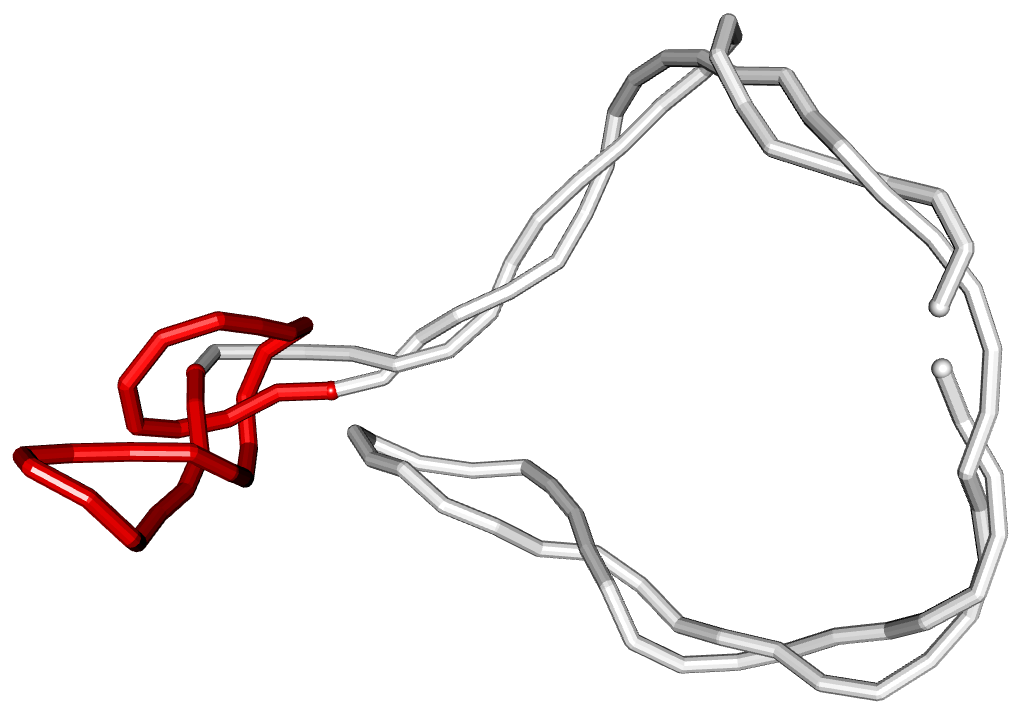
\includegraphics[width=0.7\textwidth]{3_1m_supercoiled_knotted_core_3D.png}
\caption{Piecewise linear curve given in file \lstinline{examples/3_1m_supercoiled.xyz} with knotted core highlighted in red. Figure created with script \lstinline{plot_3D_curve.R}}\label{fig:3_1m_supercoiled:knottedcore:3D}
\end{figure}



\paragraph{Closure method (subchains).}
In this last example, the polynomial invariant of each subchain was evaluated without closing the subchain (using knotoids). To evaluate the polynomial invariant of closed subchain instead (classical Jones polynomial for knots), one has to specify a closure method with the option \lstinline{--closure-method=direct} or \lstinline{--closure-method=rays}\footnote{see section ``\ref{sec:theory:knotoidsandcurves} \nameref{sec:theory:knotoidsandcurves}'' for more details.}. To evaluate the knotted core using \lstinline{rays} closure method for the subchains:
\begin{lstlisting}
$ bin/knotted_core --closure-method=rays examples/3_1m_supercoiled.xyz
\end{lstlisting}
The knotted core is written to standard output:
\begin{lstlisting}
#index_first  index_last  length  frequency  polynomial
23            51          29      0.65       - A^(-16) + A^(-12) + A^(-4)
\end{lstlisting}
To use \lstinline{direct} closure of the subchains:
\begin{lstlisting}
$ bin/knotted_core --closure-method=direct examples/3_1m_supercoiled.xyz
\end{lstlisting}
Note that with the \lstinline{direct} closure method, the polynomial does not depend on the projection. Therefore only one projection is used and the dominant knot type appears with frequency 1 (100\%):
\begin{lstlisting}
#index_first  index_last  length  frequency  polynomial
20            49          30      1          - A^(-16) + A^(-12) + A^(-4)
\end{lstlisting}

When using open subchains (\lstinline{--closure-method=open}), the polynomial invariant is evaluated after projecting the input curve on a sphere. To project on a plane, use option \lstinline{--planar}:
\begin{lstlisting}
$ bin/knotted_core --closure-method=open --planar examples/3_1m_supercoiled.xyz
\end{lstlisting}


\paragraph{Mapping polynomials to knot(oid) names.}
As with \lstinline{polynomial_invariant}, option \lstinline{--names-db} can be used to load a file mapping polynomials to knot or knotoid names
\begin{lstlisting}
$ bin/knotted_core --names-db=internal examples/3_1m_supercoiled.xyz
\end{lstlisting}
The output contains an additional column \lstinline{knotoid_type} (or \lstinline{knot_type} if subchains are closed)
\begin{lstlisting}
#index_first  index_last  length  frequency  knotoid_type  polynomial
23            52          30      0.55       3_1m          - A^(-16) + A^(-12) + A^(-4)
\end{lstlisting}
When using the special filename \lstinline{internal}, {\it Knoto-ID} uses its internal database. It is also possible to specify an external file. The directory \lstinline{examples} contains five sample files mapping polynomials to knot or knotoid names:  File \lstinline{examples/knotoid_names_sphere.txt} should be used with open subchains on the sphere 
(\lstinline{--closure-method=open} without \lstinline{--planar}, by default). For open subchains on the plane\\
(\lstinline{--closure-method=open} with \lstinline{--planar}), file \lstinline{examples/knotoid_names_planar.txt} should be used. Files  \lstinline{examples/knotoid_names_sphere_arrow.txt} and  \lstinline{examples/knotoid_names_planar_arrow.txt} should be used when working with arrow and loop arrow polynomials (with option \lstinline{--arrow-polynomial}).
When working with closed subchains (\lstinline{--closure-method=direct} or \lstinline{rays}), use file \lstinline{examples/knot_names.txt} instead.

\paragraph{Fingerprint matrices.}
By default, \lstinline{knotted_core} outputs only the knotted core to the standard output. Option \lstinline{--output} can be used to save the knotted core to a file.
While searching for the knotted core, the program computes the dominant polynomial of several subchains. These can be saved to a file using  \lstinline{--output-search}
Finally, using option \lstinline{--output-all}, the dominant polynomial is computed for every subchain and saved to a file. 
\begin{lstlisting}
$ bin/knotted_core --output-all=all.txt --output-search=search.txt --output=knotted-core.txt \
  --names-db=internal examples/3_1m_supercoiled.xyz
\end{lstlisting}
The resulting files can then be used to produce a knotoid fingerprint matrix\cite{yeates, sulkowska2012, gound} using a simple {\ttfamily R} script\cite{r2017} included with {\it Knoto-ID} 
\begin{lstlisting}
$ scripts/plot_knotted_core.R --output=fingerprint_matrix.png all.txt
\end{lstlisting}
Note that this script requires {\ttfamily R}\cite{r2017} with packages {\ttfamily optparse}\cite{optparse}, {\ttfamily ggplot2}\cite{wickham2009}, {\ttfamily reshape2}\cite{reshape2} and {\ttfamily RColorBrewer}\cite{rcolorbrewer}.
The knotted core as well as the search path can be added to the plot using options \lstinline{--knotted-core} and \lstinline{--search-path} (see Figure~\ref{fig:3_1m_supercoiled:fingerprint:search}):
\begin{lstlisting}
$ scripts/plot_knotted_core.R --output=fingerprint_matrix.png \
  --knotted-core=knotted-core.txt --search-path=search.txt all.txt
\end{lstlisting}
\begin{figure}[t]
\centering
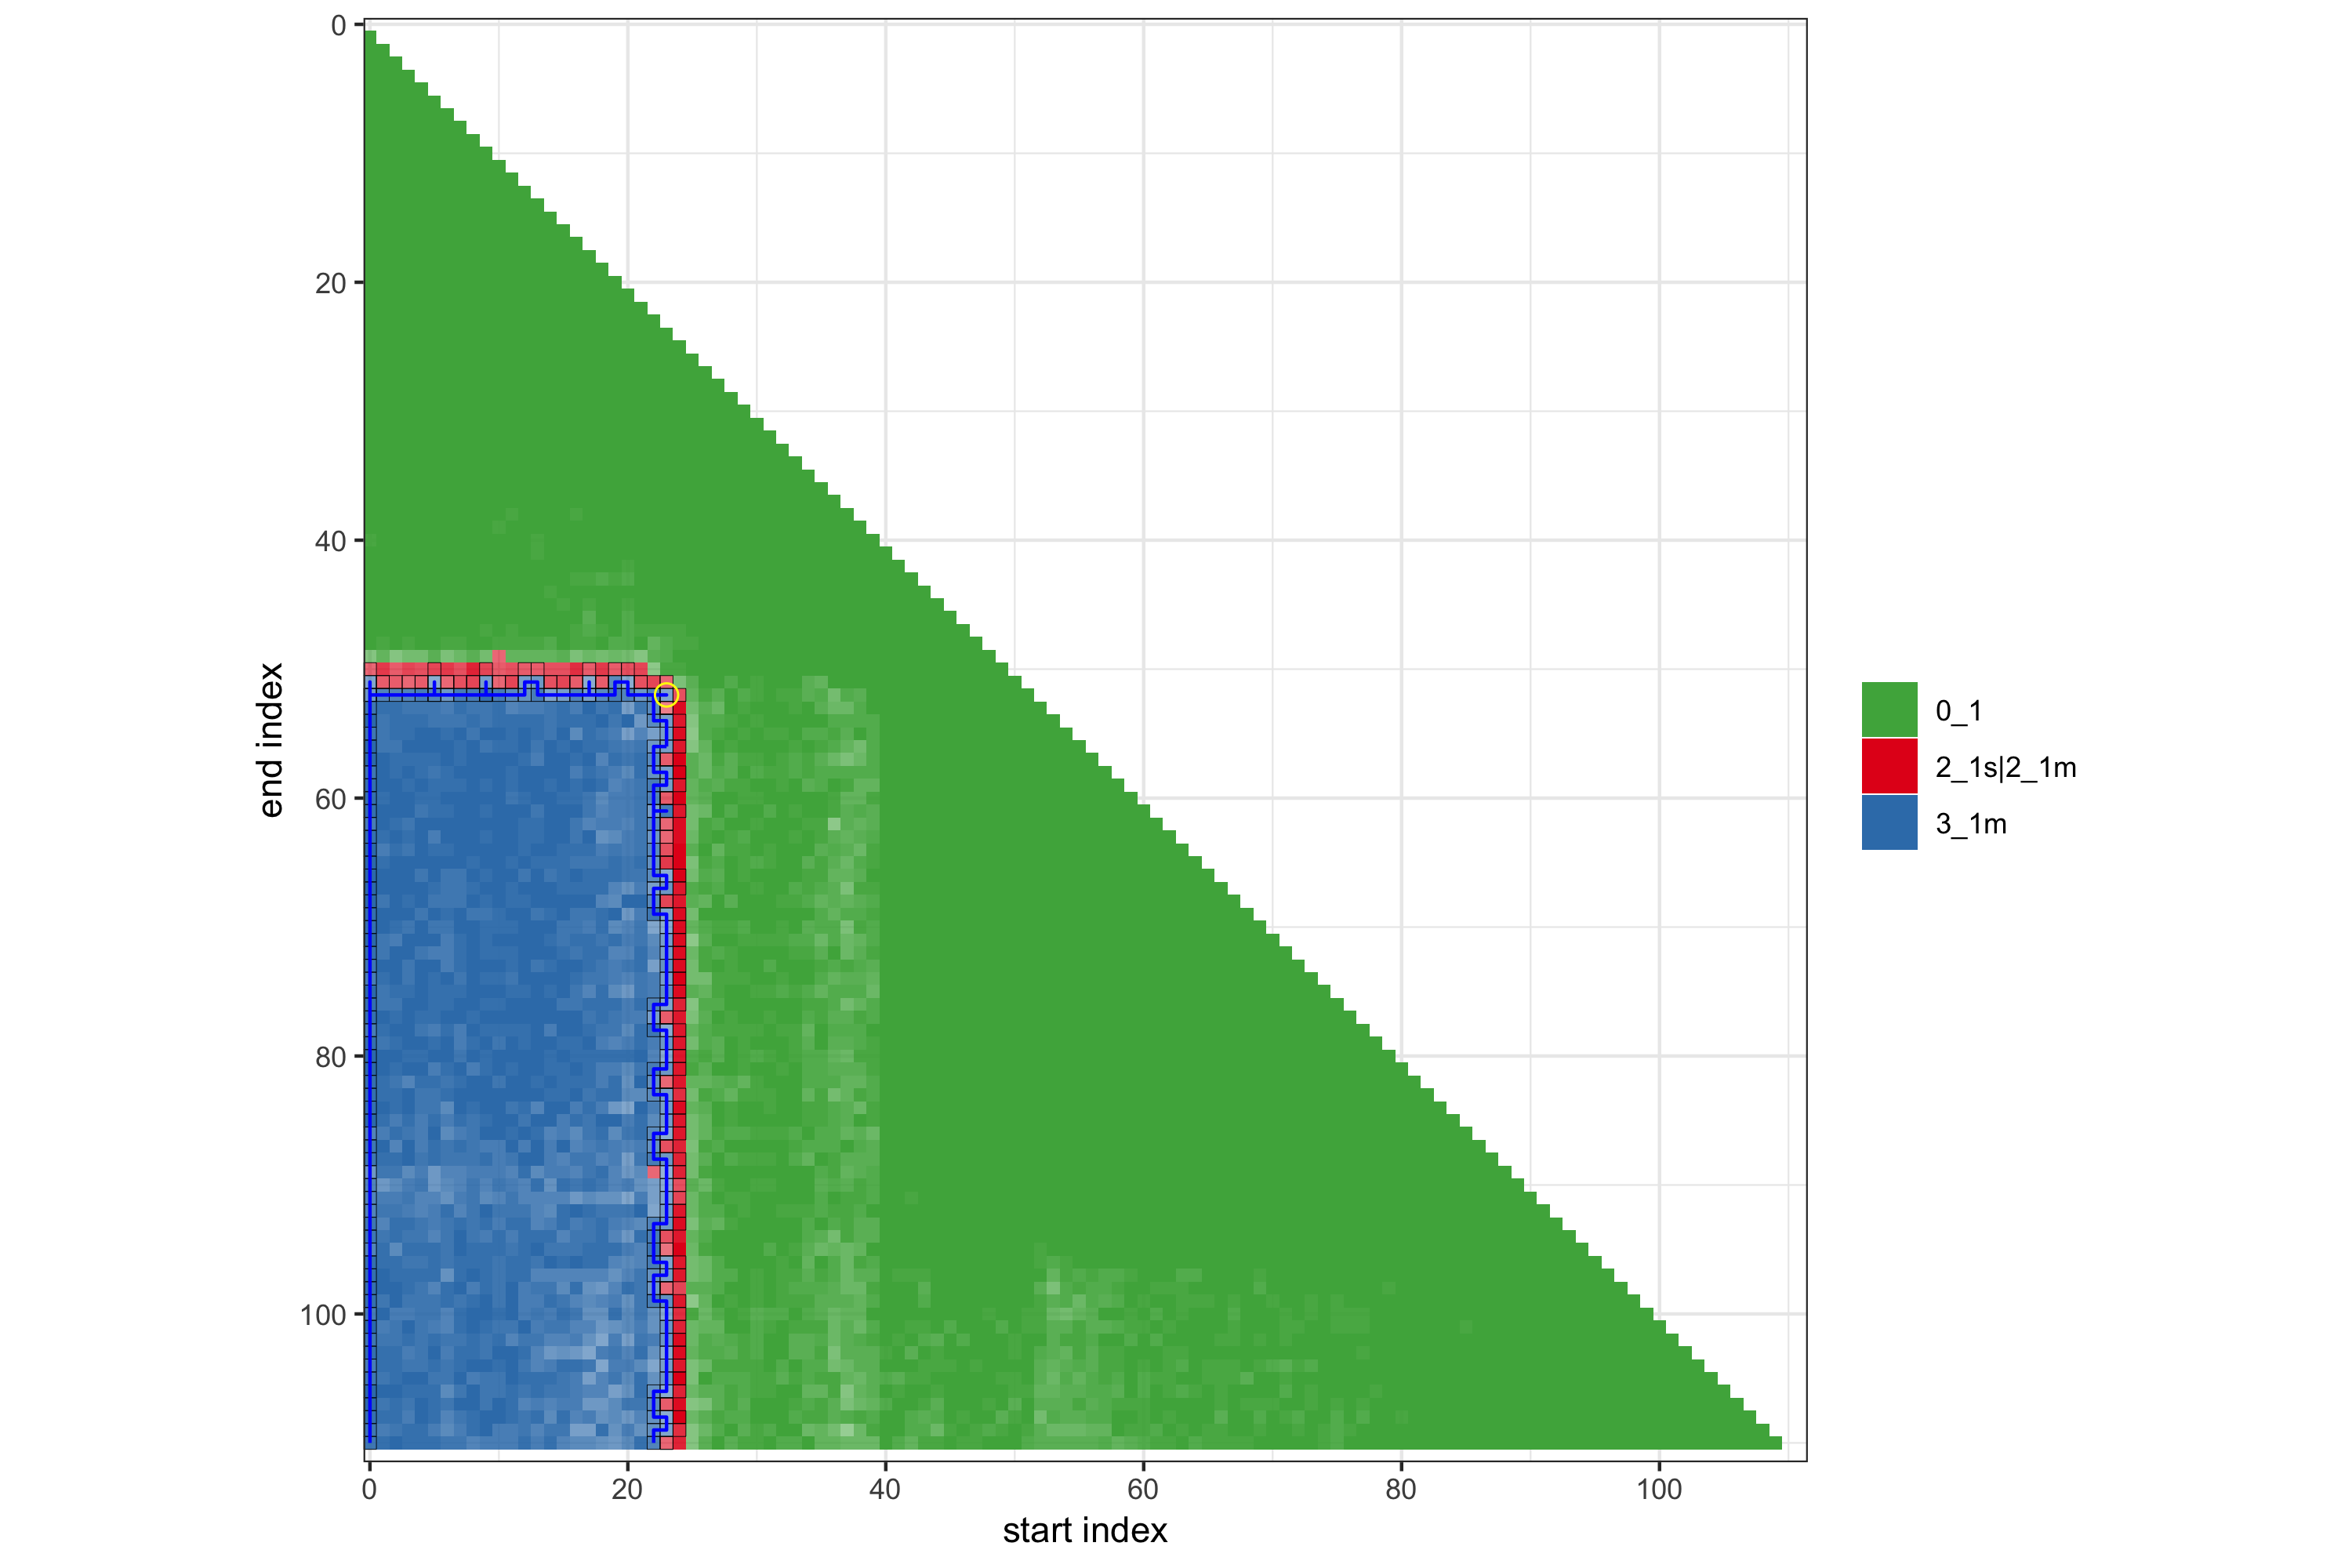
\includegraphics[width=0.9\textwidth,trim={300px 0 300px 0},clip]{3_1m_supercoiled_fingerprint_matrix_with_search.png}
\caption{ The knotoid fingerprint matrix of the curve \lstinline{examples/3_1m_supercoiled.xyz}. Each entry in this matrix with coordinates $x$ and $y$ corresponds to a subchain having start index $x$ and end index $y$. Color corresponds to the dominant knotoid type of the subchain and transparency corresponds to its frequency. The knotted core is shown with yellow circle. All subchains evaluated while searching for the knotted core are shown with a black border. In addition, the blue line shows consecutive subchains with same polynomial as the input curve that were found during the search.}\label{fig:3_1m_supercoiled:fingerprint:search}
\end{figure}
It is also possible to plot only the search path by replacing the file \lstinline{all.txt} by \lstinline{search.txt}:
\begin{lstlisting}
$ scripts/plot_knotted_core.R --output=fingerprint_matrix.png \
  --knotted-core=knotted-core.txt search.txt
\end{lstlisting}

\paragraph{Projections.}
By default \lstinline{knotted_core} uses 20 projections\footnote{randomly chosen with uniform distribution on the surface of the sphere.} to estimate the dominant knot(oid). The number of random projection can be changed with \lstinline{--nb-projections}. For example, to use 100 projections:
\begin{lstlisting}
$ bin/knotted_core --nb-projections=100 examples/3_1m_supercoiled.xyz
\end{lstlisting}
Alternatively, a predefined list of projections can be specified with option \lstinline{--projections-list}. For example to use the list of projections given in file \lstinline{examples/projections_list_100.txt}:
\begin{lstlisting}
$ bin/knotted_core --projections-list=examples/projections_list_100.txt examples/3_1m_supercoiled.xyz
\end{lstlisting}

The number of projections has an impact on computational cost (proportional to the number of projections) but also on the precision of the results. 
Figure~\ref{fig:3_1m_supercoiled:fingerprint:nprojections} presents fingerprint matrices of the curve \lstinline{examples/3_1m_supercoiled.xyz} obtained with different number of projections. The fingerprint matrix obtained with \lstinline{--nb-projections=1} is very noisy, with multiple spurious dominant knotoid types. With \lstinline{--nb-projections=10} the matrix already gives a good approximation at a reasonable computational cost. With \lstinline{--nb-projections=100} the level of noise is strongly decreased and all the spurious knotoid types disappear.
\begin{figure}[t]
\centering
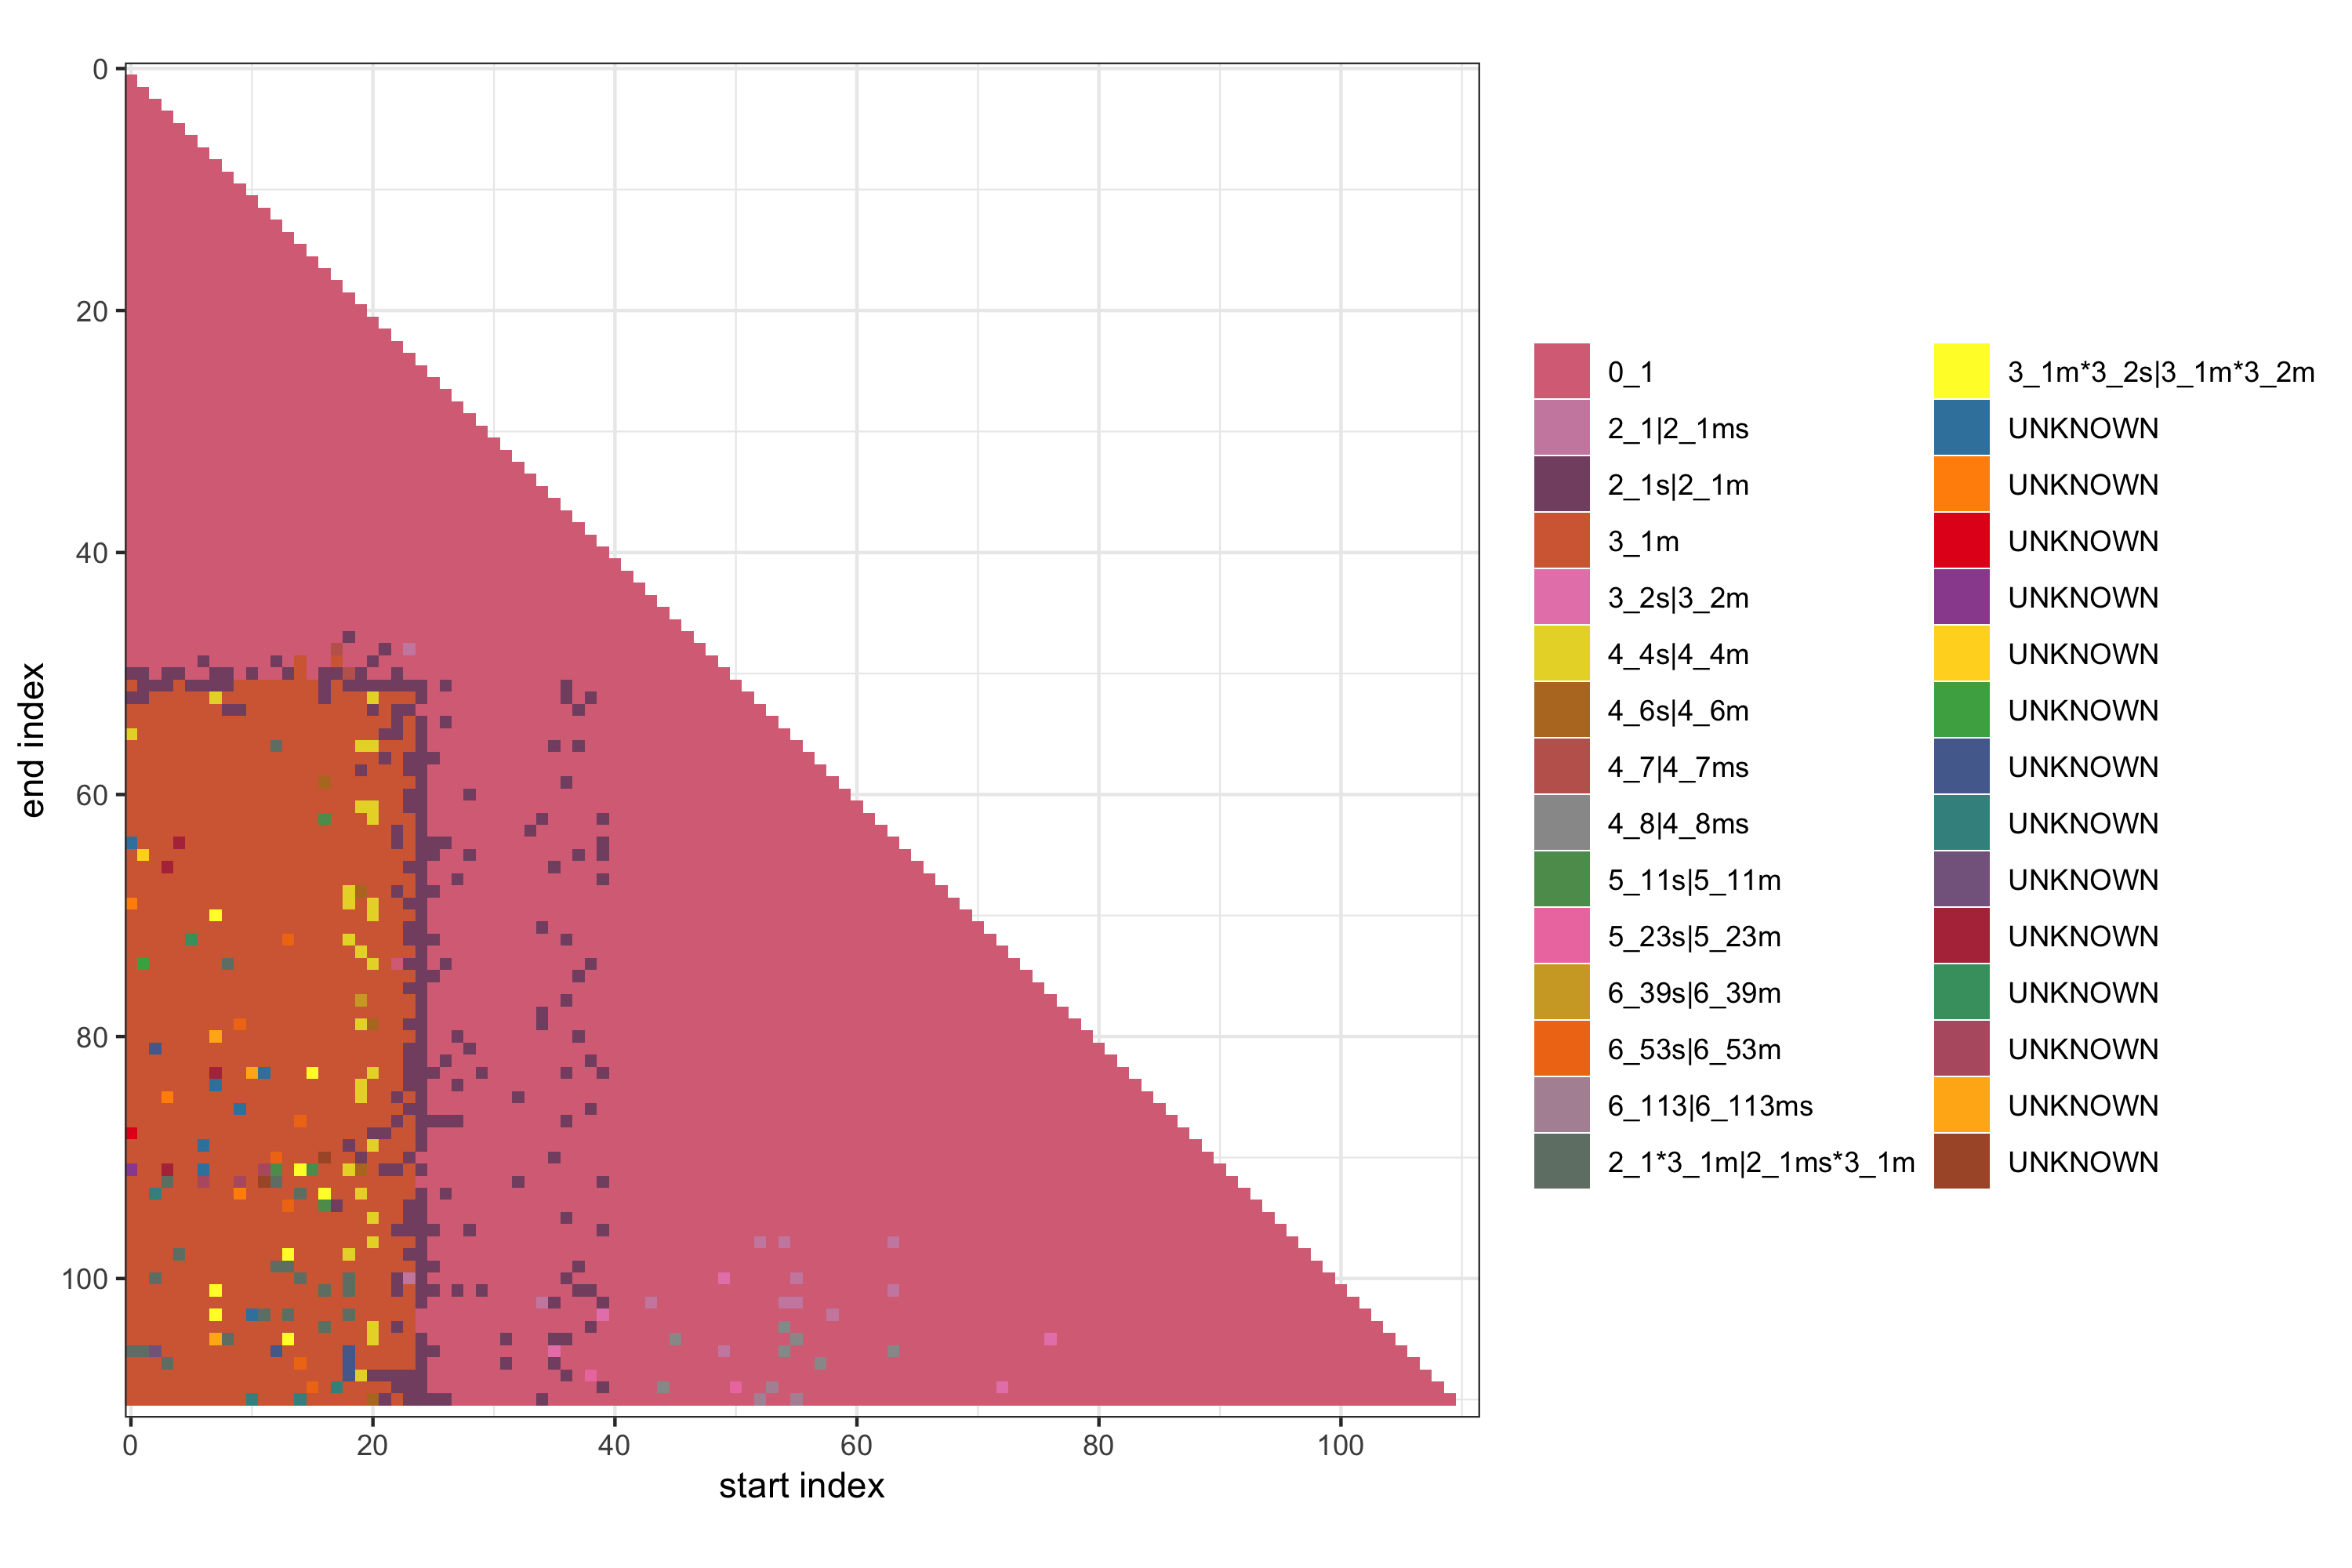
\includegraphics[width=0.39\textwidth]{3_1m_supercoiled_fingerprint_matrix_1.png}
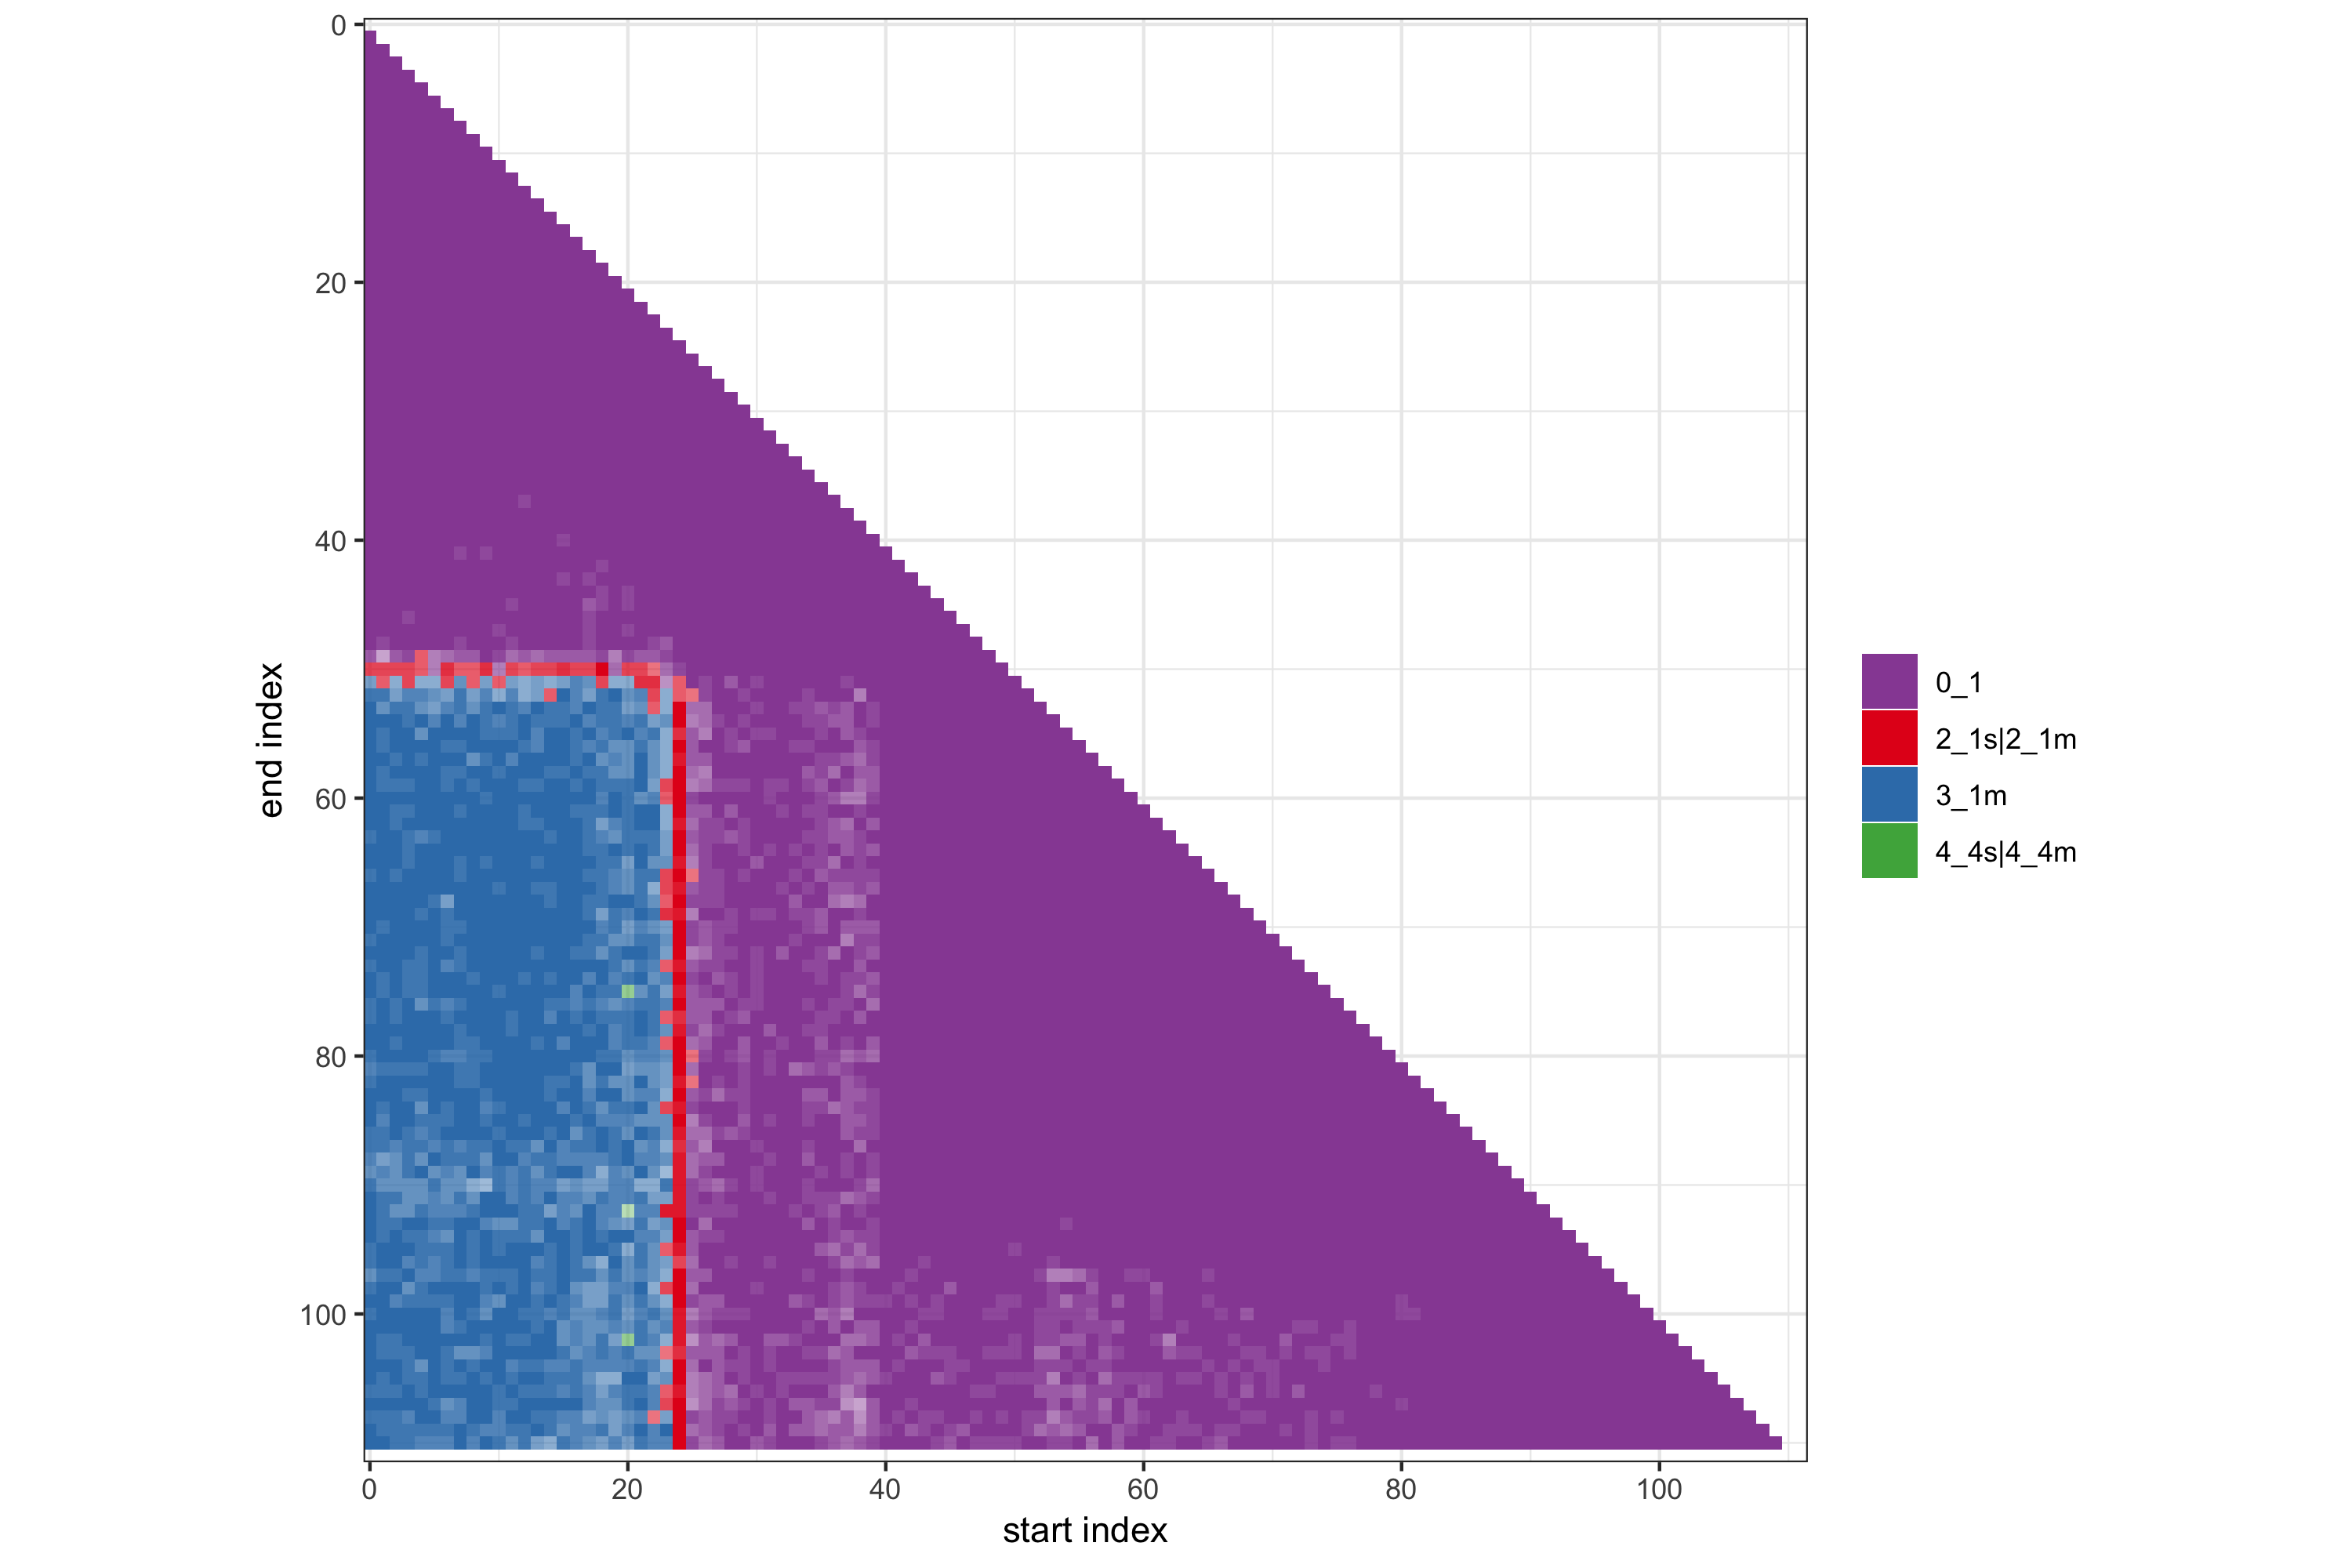
\includegraphics[width=0.29\textwidth,trim={300px 0 300px 0},clip]{3_1m_supercoiled_fingerprint_matrix_10.png}
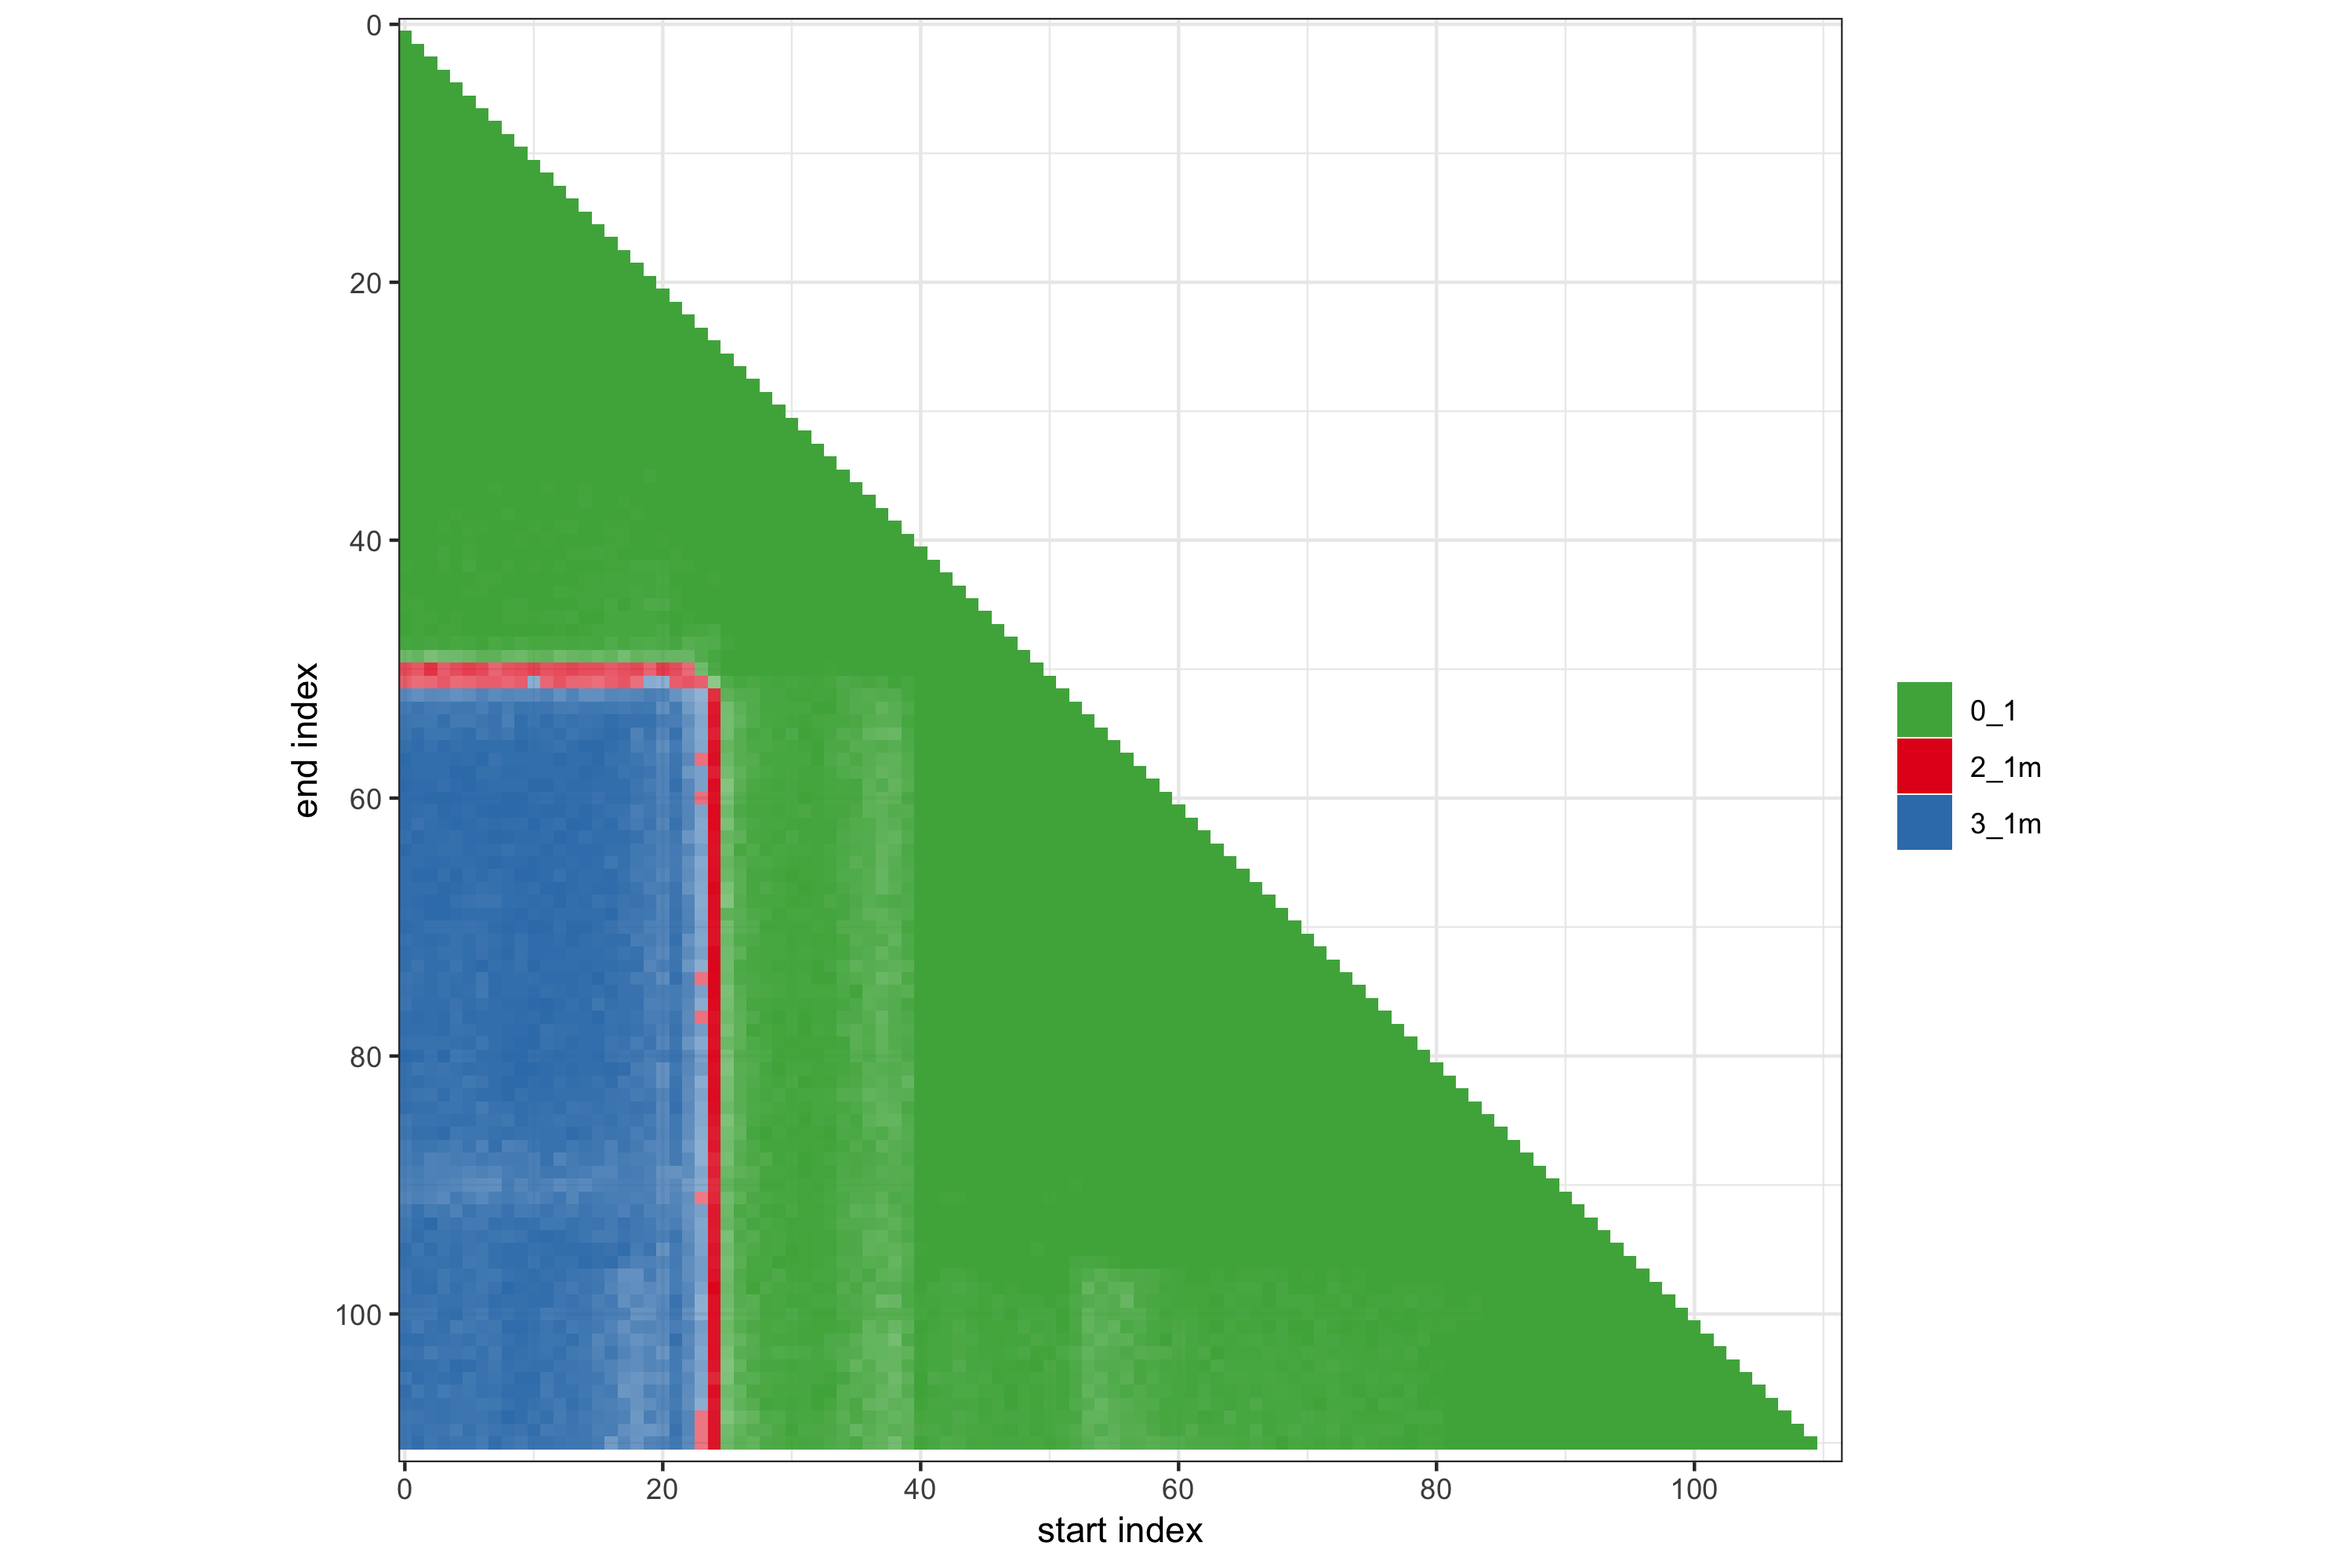
\includegraphics[width=0.29\textwidth,trim={300px 0 300px 0},clip]{3_1m_supercoiled_fingerprint_matrix_100.png}
\caption{ The knotoid fingerprint matrix of the curve \lstinline{examples/3_1m_supercoiled.xyz} obtained with 1 projection (left), 10 projections (middle) and 100 projections (right).}\label{fig:3_1m_supercoiled:fingerprint:nprojections}
\end{figure}



\subsubsection{Using closed curves as input}
By default, the input curve is considered as open. To close the input curve with a straight line from last to first point, use option \lstinline{--cyclic-input}:
\begin{lstlisting}
$ bin/knotted_core --cyclic-input examples/3_1m_supercoiled.xyz
\end{lstlisting}
When using option \lstinline{--cyclic-input}, the input curve is closed with direct closure\footnote{closed with a straight line from last to first point of the curve.}. Therefore, this option should be used with caution and one should make sure that endpoints are close enough so that direct closure does not disturb the topology of the input curve. Note that the direct closure method used to close the input curve (\lstinline{--cyclic-input}) is completely independent from the choice of closure method for the subchains (\lstinline{--closure-method}).

Closing the input curve modifies the set of possible subchains that are considered when searching for the knotted core.
With open input curve, subchains were not allowed to contain endpoints of the input curve (except at their endpoint).
When an input curve is closed, the first and last points are not endpoints anymore and can appear anywhere in the subchains (see Figure~\ref{fig:subchains}).
\begin{figure}[t]
\centering
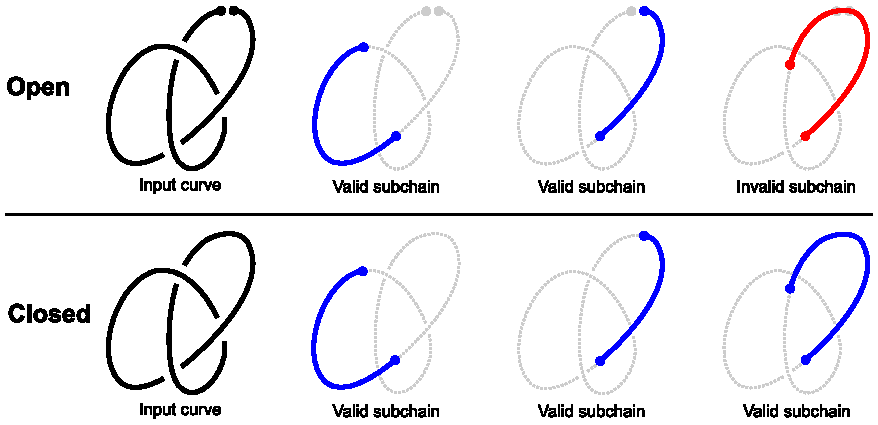
\includegraphics[width=1\textwidth]{subchains.pdf}
\caption{With open input curve (upper panel), subchains are not allowed to contain endpoints of the input curve (except at their endpoint). With closed input curve (lower panel), all subchains are allowed. Example of valid subchains are shown in blue, and invalid subchain in red. }\label{fig:subchains}
\end{figure}

With closed input curves, one should be careful when interpreting the output of \lstinline{knotted_core}. Indeed, in the output of \lstinline{knotted_core}\footnote{see section ``\ref{sec:format:listsubchains} \nameref{sec:format:listsubchains}'' for more information on the file format.}, subchains are defined by two points of the input curve (\lstinline{index_first} and \lstinline{index_last}). When the first point has an index $i_1$ lower than the last point $i_2$, the subchain consist of all points with indices: $\{i_1,i_1+1,i_1+2,\cdots,i_2\}$.
However, when the first point has an index $i_1$ higher than the last point $i_2$, the subchain consist of all points with index larger or equal to the index of the first point up to the last point of the input curve, and then continue with the first point of the input curve up to $i_2$, i.e. for an input curve with $N$ points (using zero-based indexing): $\{i_1,i_1+1,i_1+2,\cdots,N-1,0,1,2,\cdots,i_2\}$. For example, the output
\begin{lstlisting}
#index_first  index_last  length  frequency  polynomial
3             8           6      0.5       - A^(-16) + A^(-12) + A^(-4)
\end{lstlisting}
corresponds to the subchain with points $\{3,4,5,6,7,8\}$ of the input curve, while 
\begin{lstlisting}
#index_first  index_last  length  frequency  polynomial
109           3           6      0.5       - A^(-16) + A^(-12) + A^(-4)
\end{lstlisting}
corresponds to the subchain with points $\{109,110,0,1,2,3\}$ of the input curve (which has 111 points).

All options discussed when using open input curve can also be used with closed curve. In particular, the option \lstinline{--closure-method}, which defines how each subchain should be closed (or kept open), can be used independently from the choice of closure for the input curve (\lstinline{--cyclic-input}). For example, to evaluate the knotted core of the closed input curve \lstinline{examples/3_1m_supercoiled.xyz} based on the evaluation of the polynomial invariant of open subchains projected on the sphere (Jones polynomial for knotoids):
\begin{lstlisting}
$ bin/knotted_core --output-all=all.txt --output-search=search.txt --output=knotted-core.txt \
  --names-db=internal --nb-projections=100 --cyclic-input \
  examples/3_1m_supercoiled.xyz
\end{lstlisting}
The resulting knotted core is saved in the file \lstinline{knotted-core.txt}, while the dominant knotoid types of all possible subchains and of all subchains evaluated during the search are saved in files \lstinline{all.txt} and \lstinline{search.txt} respectively.


The resulting files can be used to produce a disk matrix\cite{rawdon} 
with \lstinline{plot_knotted_core.R} and option \lstinline{--cyclic} (see Figure~\ref{fig:3_1m_supercoiled:disk}):
\begin{lstlisting}
$ scripts/plot_knotted_core.R --cyclic --output=disk_matrix.png \
  --knotted-core=knotted-core.txt all.txt
\end{lstlisting}
\begin{figure}[t]
\centering
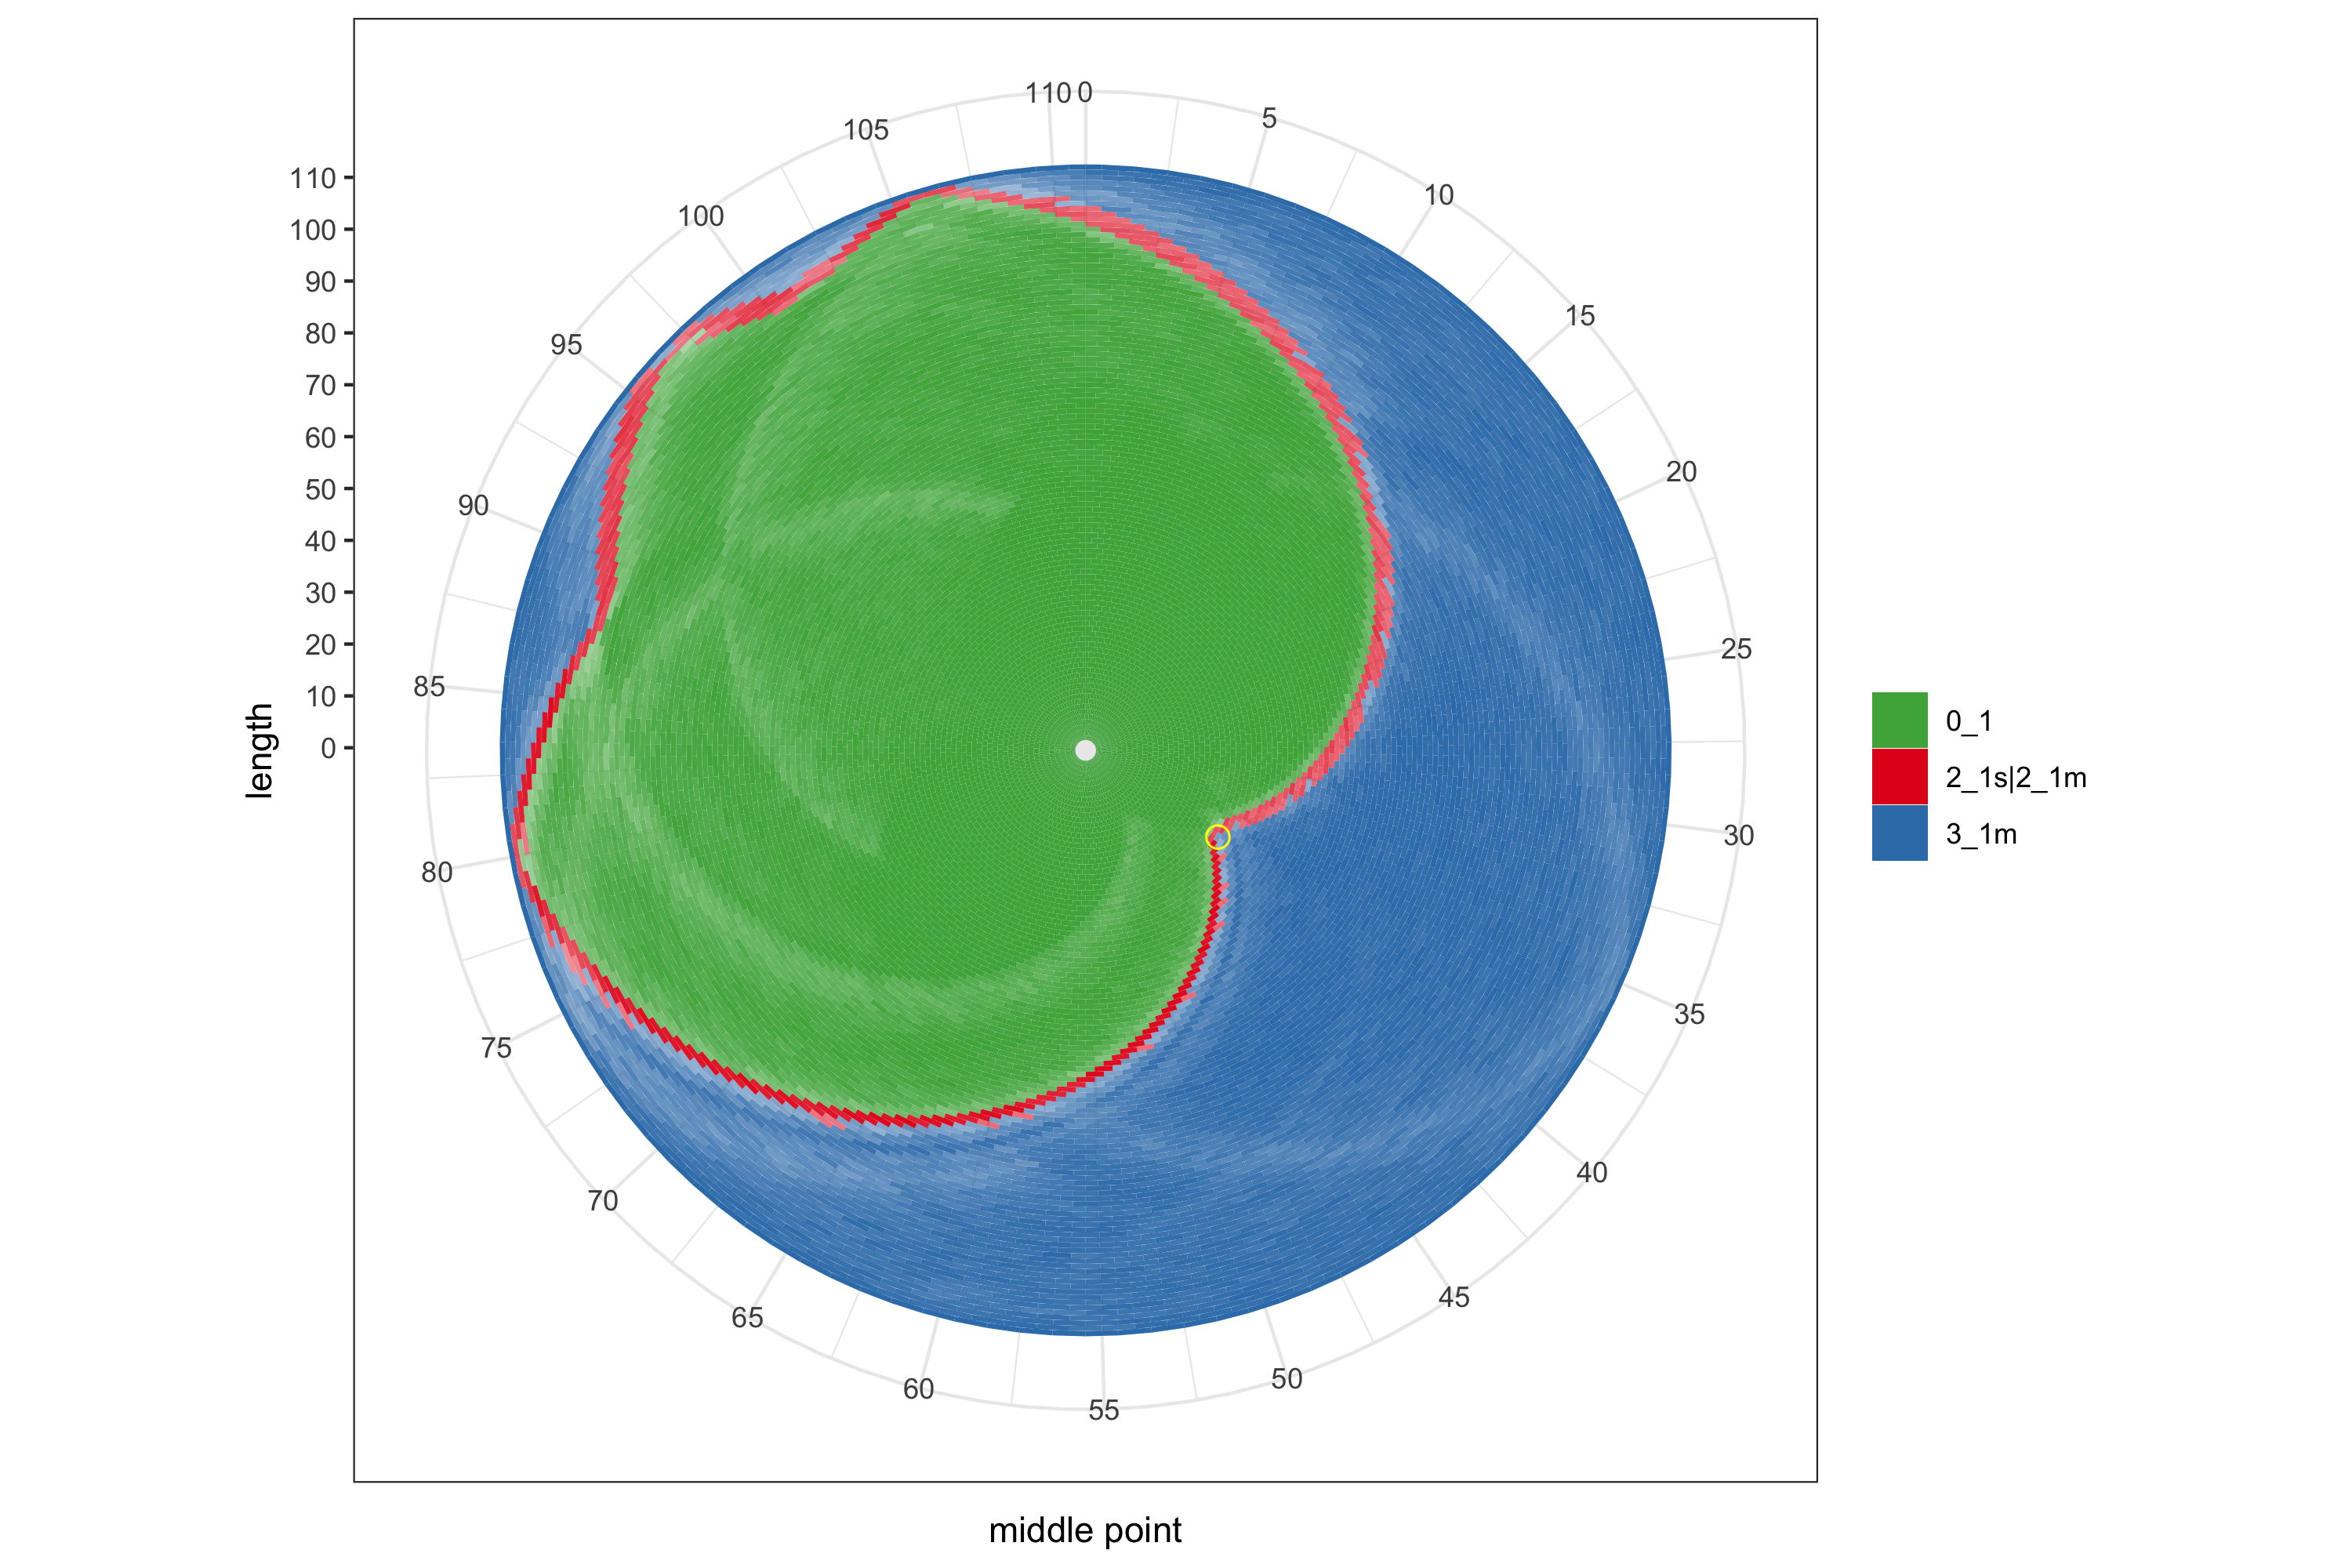
\includegraphics[width=0.9\textwidth,trim={300px 0 300px 0},clip]{3_1m_supercoiled_disk_matrix.png}
\caption{ The disk matrix of the closed curve \lstinline{examples/3_1m_supercoiled.xyz}. Radial coordinate corresponds to the length of the subchain and angular coordinate to the midpoint of the subchain. Color corresponds to dominant knotoid type of the subchain and transparency to its frequency. The knotted core is shown with a yellow circle.}\label{fig:3_1m_supercoiled:disk}
\end{figure}



\clearpage
\subsection{\label{sec:example}Real life example: protein 3KZN}
In this section we apply the concepts discussed above on a real life example.
\subsubsection{Knotoids}
We start by downloading the protein structure that we want to analyze from the Protein database (PDB)\cite{pdb}. In this example we shall use the protein 3KZN\cite{shi2006} that is known to form a deep trefoil knot.
\begin{lstlisting}
$ wget https://files.rcsb.org/download/3KZN.pdb
\end{lstlisting}
Note for Windows users: with the {\it Windows PowerShell}, \lstinline{wget} needs the additional option \lstinline{-OutFile 3KZN.pdb}. Alternatively, the file \lstinline{https://files.rcsb.org/download/3KZN.pdb} can be simply downloaded using a web browser.

The next step is to extract from the .pdb file the $xyz$-coordinates of the $C_\alpha$ atoms, that make up the protein backbone and store them into a file with xyz file format\footnote{see section ``\ref{sec:format:xyz} \nameref{sec:format:xyz}'' for more information on the file format.}. Note that a protein molecule may include more than one chains in its conformation so one has to be careful when extracting coordinates. In this example we work with chain $A$.
Note that many proteins that are deposited in the PDB have gaps in their conformations. If this is the case, the gaps are connected with a straight line. One should be careful when dealing with such situations since connecting the endpoints of a gap with a straight line may alter the topology of the chain.
For further details on the .pdb file format, the reader should refer to the documentation at \url{http://www.wwpdb.org/documentation/file-format}. The simple script \lstinline{pdb_to_xyz.R}\footnote{To use this script, {\ttfamily R}\cite{r2017} must be installed with packages {\ttfamily optparse}\cite{optparse} and {\ttfamily Rpdb}\cite{rpdb}.} distributed with {\it Knoto-ID} can be used to convert the pdb file \lstinline{3KZN.pdb} to xyz format and save the output to \lstinline{examples/3KZN_chain_A.xyz}:
\begin{lstlisting}
$ scripts/pdb_to_xyz.R --output=examples/3KZN_chain_A.xyz 3KZN.pdb
\end{lstlisting}

We can evaluate the Jones polynomial for knotoids on the sphere of this protein chain by calling the command:
\begin{lstlisting}
$ bin/polynomial_invariant examples/3KZN_chain_A.xyz 
\end{lstlisting}
which generates the following output to standard error:
\begin{lstlisting}
seed: 1501677085
polynomial invariant: Jones polynomial for knotoids.
Loading input curve
3D curve has 331 vertices
projection: -0.443782,-0.690045,-0.571748
Simplifying 3D curve
3D curve has 13 vertices
Evaluating diagram
diagram has 8 crossings
Simplifying diagram
diagram has 5 crossings
Simplifying diagram with random reidemeister moves III (max 100000 moves)
diagram has 5 crossings
Final simplifying diagram
diagram has 5 crossings
\end{lstlisting}
As we can see, the output includes information, amongst other things, on the random projection that was used and an upper bound on the crossing number of the diagram. After completion, the Jones polynomial for knotoids of the chain is written to standard output:
\begin{lstlisting}
Polynomial:  - A^(-16) + A^(-12) + A^(-4)
\end{lstlisting}
For the moment, we don't have any information on the knotoid type that corresponds to this polynomial. However, this can be solved easily by using the option \lstinline{--names-db} to specify a knotoid names database:
\begin{lstlisting}
$ bin/polynomial_invariant --projection="-0.443782,-0.690045,-0.571748" \
  --names-db=internal examples/3KZN_chain_A.xyz
\end{lstlisting}
We have used the option \lstinline{--projection} in order to use a fixed projection for our chain. In particular, we used the projection that was randomly chosen in the previous run. The option \lstinline{--names-db=internal} allows the loading of the internal knot(oid)s names database. Instead of the keyword \lstinline{internal}, an external file specifying the mapping from polynomials to names can also be given\footnote{see section ``\ref{sec:format:namesdb} \nameref{sec:format:namesdb}'' for more information on the file format.}. The standard output now takes the following form:
\begin{lstlisting}
Knotoid type: 3_1m      Polynomial:  - A^(-16) + A^(-12) + A^(-4)
\end{lstlisting}
This means that this particular projection of the protein chain corresponds to a knot-type knotoid with 3 crossings. As mentioned in section ``\ref{sec:theory} \nameref{sec:theory}'', the chain is considered lying inside a large enough sphere. Each point of the sphere indicates a projection direction towards an oriented surface that lies outside the sphere that encloses the chain. There are two options for the oriented surface: a sphere, which is the default option and is the one that was used so far in this example, as well as the 2D plane. By adding the option \lstinline{--planar}, we evaluate the knotoid type of the protein chain using planar knotoids.
\begin{lstlisting}
$ bin/polynomial_invariant --projection="-0.443782,-0.690045,-0.571748" \
  --names-db=internal --planar examples/3KZN_chain_A.xyz
\end{lstlisting}
In this case the knotoid type of the protein chain remains the same upon evaluation using planar knotoids. Indeed
\begin{lstlisting}
Knotoid type: 3_1m      Polynomial:  - A^(-16) + A^(-12) + A^(-4)
\end{lstlisting}
Note that this is not the general case. There could be protein chains that have a planar knotoid type different from the knotoid type on the sphere.

To evaluate the arrow polynomial for knotoids on the sphere instead of the Jones polynomial, use option\\
\lstinline{--arrow-polynomial}:
\begin{lstlisting}
$ bin/polynomial_invariant --projection="-0.443782,-0.690045,-0.571748" \
  --names-db=internal --arrow-polynomial examples/3KZN_chain_A.xyz
\end{lstlisting}
To evaluate the loop arrow polynomial for knotoids on the plane instead of the Turaev loop bracket polynomial, use option \lstinline{--arrow-polynomial} together with \lstinline{--planar}:
\begin{lstlisting}
$ bin/polynomial_invariant --projection="-0.443782,-0.690045,-0.571748" \
  --names-db=internal --planar --arrow-polynomial examples/3KZN_chain_A.xyz
\end{lstlisting}
In this specific example, using arrow or loop arrow polynomial gives the same result as the Jones polynomial for knotoid and Turaev loop bracket polynomial.


In the example runs that we presented so far, the results were just printed to standard output. By adding the option \lstinline{--output=FILENAME}, we can ask the program to print the results into a file. Moreover, by including \lstinline{--output-diagram=FILENAME} the program creates a separate file that contains the corresponding knotoid diagram in PD format\footnote{see section ``\ref{sec:format:pd} \nameref{sec:format:pd}'' for more information on the file format.}:
\begin{lstlisting}
$ bin/polynomial_invariant --projection="-0.443782,-0.690045,-0.571748" \
  --names-db=internal --planar --output-diagram=3KZN_diagram.txt \ 
  --output=3KZN_polynomial.txt examples/3KZN_chain_A.xyz
\end{lstlisting}
Note that option \lstinline{--output-diagram-format=gauss} can be used to output extended Gauss codes\footnote{see section ``\ref{sec:format:gauss} \nameref{sec:format:gauss}'' for more information on the file format.} instead of PD codes for the knotoid diagrams.

Up until this point, we have dealt only with a single projection of the protein chain. In order to find the dominant knotoid type of a chain, we have to consider all of its projections and, subsequently, sample them in a uniform way. By adding the option \lstinline{--nb-projections=N} the program samples ${\rm N}$ random projections with uniform distribution on the surface of the sphere. Below we give an example with 100 random projections:
\begin{lstlisting}
$ bin/polynomial_invariant --nb-projections=100 --names-db=internal \
  --planar examples/3KZN_chain_A.xyz
\end{lstlisting}
The standard output includes a histogram of frequency of appearance of knotoid types. The knotoid with the highest frequency of appearance is the dominant knotoid type of the chain:
\begin{lstlistingsmall}
#frequency knotoid_type    polynomial
0.63       3_1m                       - A^(-16) + A^(-12) + A^(-4)
0.07       UNKNOWN                    - A^(-30)*v - 2*A^(-28) - A^(-28)*v - 2*A^(-26) + A^(-26)*v + A^(-24) + ...
0.07       1_1*3_1m                   + A^(-14)*v + A^(-12) - A^(-10)*v - A^(-8) - A^(-2)*v - 1
0.04       2_4s*3_1m|2_4m*3_1m        - A^(-24)*v - 2*A^(-22) - A^(-20) + A^(-20)*v + 2*A^(-18) + A^(-16) + A^...
0.04       4_4s|4_4m                  - A^(-18) - A^(-16) + A^(-14) + 2*A^(-12) - A^(-8) + A^(-4)
0.04       2_1s*3_1m|2_1m*3_1m        + A^(-26) - 2*A^(-22) - A^(-20) + A^(-18) + A^(-16) - A^(-14) + A^(-10) ...
0.03       2_6*3_1m                   + A^(-20) - A^(-16) - A^(-16)*v^(2) - A^(-14)*v + A^(-12)*v^(2) + A^(-10...
0.02       UNKNOWN                    + A^(-22) + A^(-20) + A^(-20)*v + A^(-18)*v - A^(-16) - A^(-16)*v - A^(-...
0.01       UNKNOWN                    - A^(-14) - A^(-12) - A^(-12)*v - A^(-10) - A^(-10)*v + A^(-8)*v + 2*A^(...
0.01       UNKNOWN                    - A^(-14) - A^(-12) + 2*A^(-8) + 2*A^(-6) - A^(-2)
0.01       4_46|4_46ms                - A^(-12) - A^(-10) - A^(-10)*v + A^(-6) + A^(-6)*v + A^(-4) - A^(-2)*v - 1
0.01       2_1*3_1m|2_1ms*3_1m        - A^(-12) - A^(-10) + A^(-8) + 2*A^(-6) - A^(-2) + 1 + A^(2) - A^(6)
0.01       5_81|5_81ms|5_316|5_316ms  - A^(-10) + A^(-6) - A^(-2) - A^(-2)*v - 1 - v - A^(2)
0.01       2_5*3_1m                   + A^(-14)*v - 2*A^(-10)*v - A^(-8) + A^(-6)*v + A^(-4) - A^(-2)*v + A^(2...
\end{lstlistingsmall}
In this example, the dominant knotoid type for the protein 3KZN is the knot-type knotoid $3_1m$ with frequency of appearance 63\%. Note that the exact frequency may change depending on the 100 random projections chosen. If multiple knotoid types have the same polynomial invariant\footnote{in the knotoid names database specified with \lstinline{--names-db}.}, all knotoid types are concatenated with a \lstinline{|} separator. \lstinline{UNKNOWN} corresponds to knotoids not found in the database (more than 5 crossings).

We can also use a predetermined list of projections. In the following example we use the option \lstinline{--projections-list} in order to specify a list of 100 fixed projection directions uniformly distributed on the surface of a sphere, weighted by the surface of their corresponding Voronoi cells\footnote{see section ``\ref{sec:format:projections} \nameref{sec:format:projections}'' for a description of the file format.}. 
\begin{lstlisting}
$ bin/polynomial_invariant --projections-list=examples/projections_list_100.txt \
  --names-db=internal --planar examples/3KZN_chain_A.xyz
\end{lstlisting}

Using option \lstinline{--output-diagram=diagrams.txt}, the list of projection directions with corresponding polynomials and knotoid types is saved to file \lstinline{diagrams.txt}. Although 100 projection can be sufficient to obtain a first approximation of the projection map, better results can be achieved using a larger number of projections:
\begin{lstlisting}
$ bin/polynomial_invariant --nb-projections=10000 --names-db=internal \
  --planar --output-diagram=diagrams.txt examples/3KZN_chain_A.xyz
\end{lstlisting}
The script \lstinline{plot_projection_map.R} can then be used to plot the projection map using voronoi tesselation:
\begin{lstlisting}
$ scripts/plot_projection_map.R --output=projection_map.png diagrams.txt
\end{lstlisting}
The resulting projection map is shown in Figure~\ref{fig:3KZN:projectionmap}.
\begin{figure}[t]
\centering
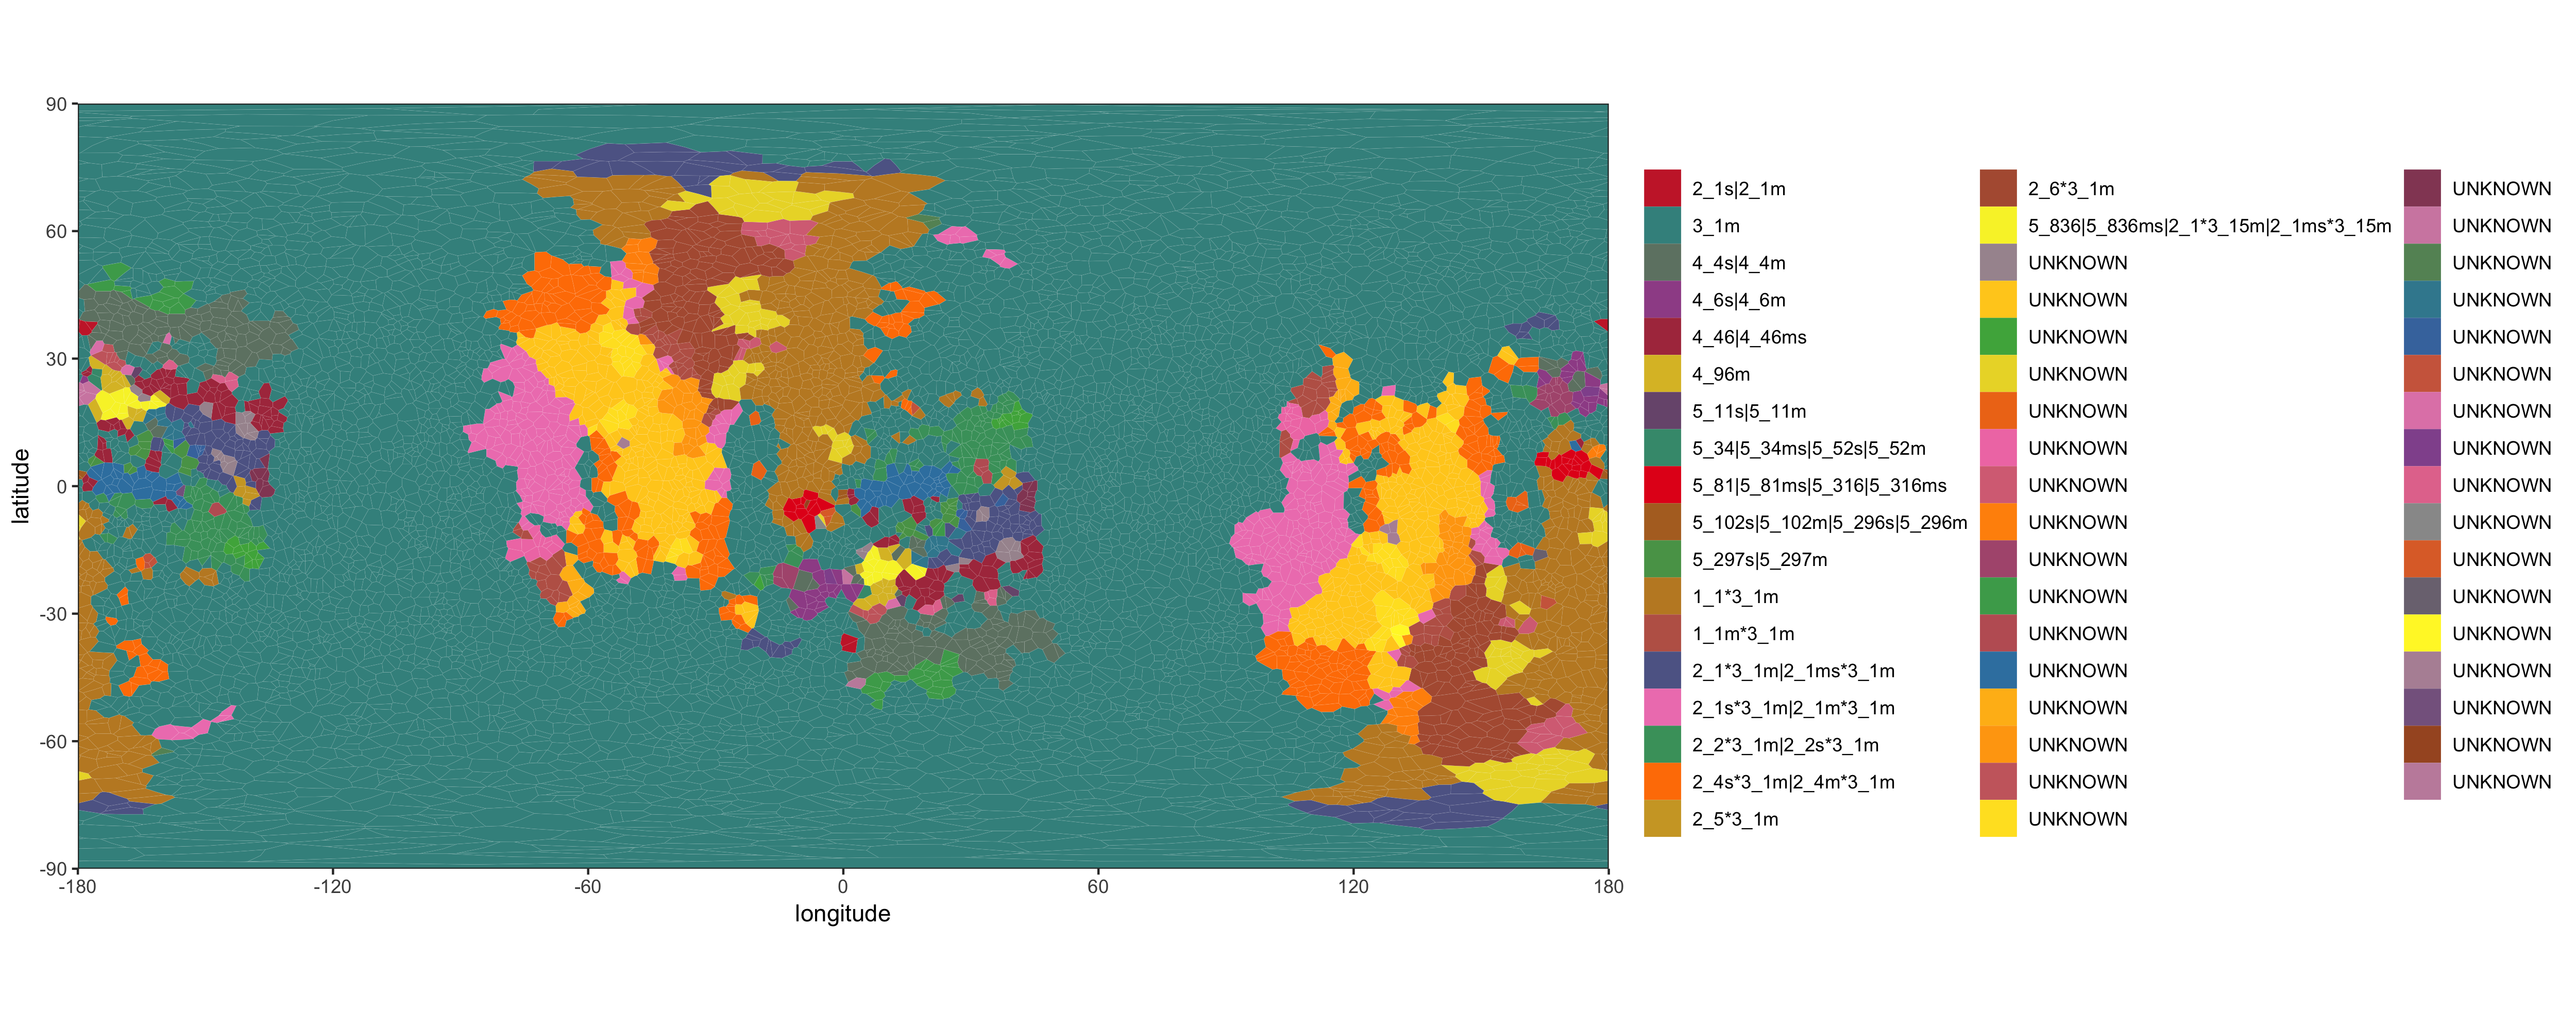
\includegraphics[width=1\textwidth]{3KZN_projection_map.png}
\caption{Projection map for the protein 3KZN (obtained with 10000 projections).  For a projection direction $(x,y,z)$, longitude ($\lambda$) and latitude ($\delta$) are defined as $x=\cos(\delta)\cos(\lambda)$, $y=\cos(\delta)\sin(\lambda)$, $z=\sin(\delta)$. Colors correspond to planar knotoid types. Since the voronoi tesselation is performed on the sphere, voronoi facets are separated by arcs of great circles, which do not correspond to straight line after equirectangular projection.}\label{fig:3KZN:projectionmap}
\end{figure}
The script \lstinline{plot_projection_map.R} can also be used to create a 3D globe (webGL) with the backbone of the protein using options \lstinline{--output-3D} and \lstinline{--curve-3D}:
\begin{lstlisting}
$ scripts/plot_projection_map.R --output=projection_map.png --output-3D=projection_map.html \
  --curve-3D=examples/3KZN_chain_A.xyz diagrams.txt
\end{lstlisting}
A screenshot is shown in Figure~\ref{fig:3KZN:projectionmap:3D}.
\begin{figure}[t]
\centering
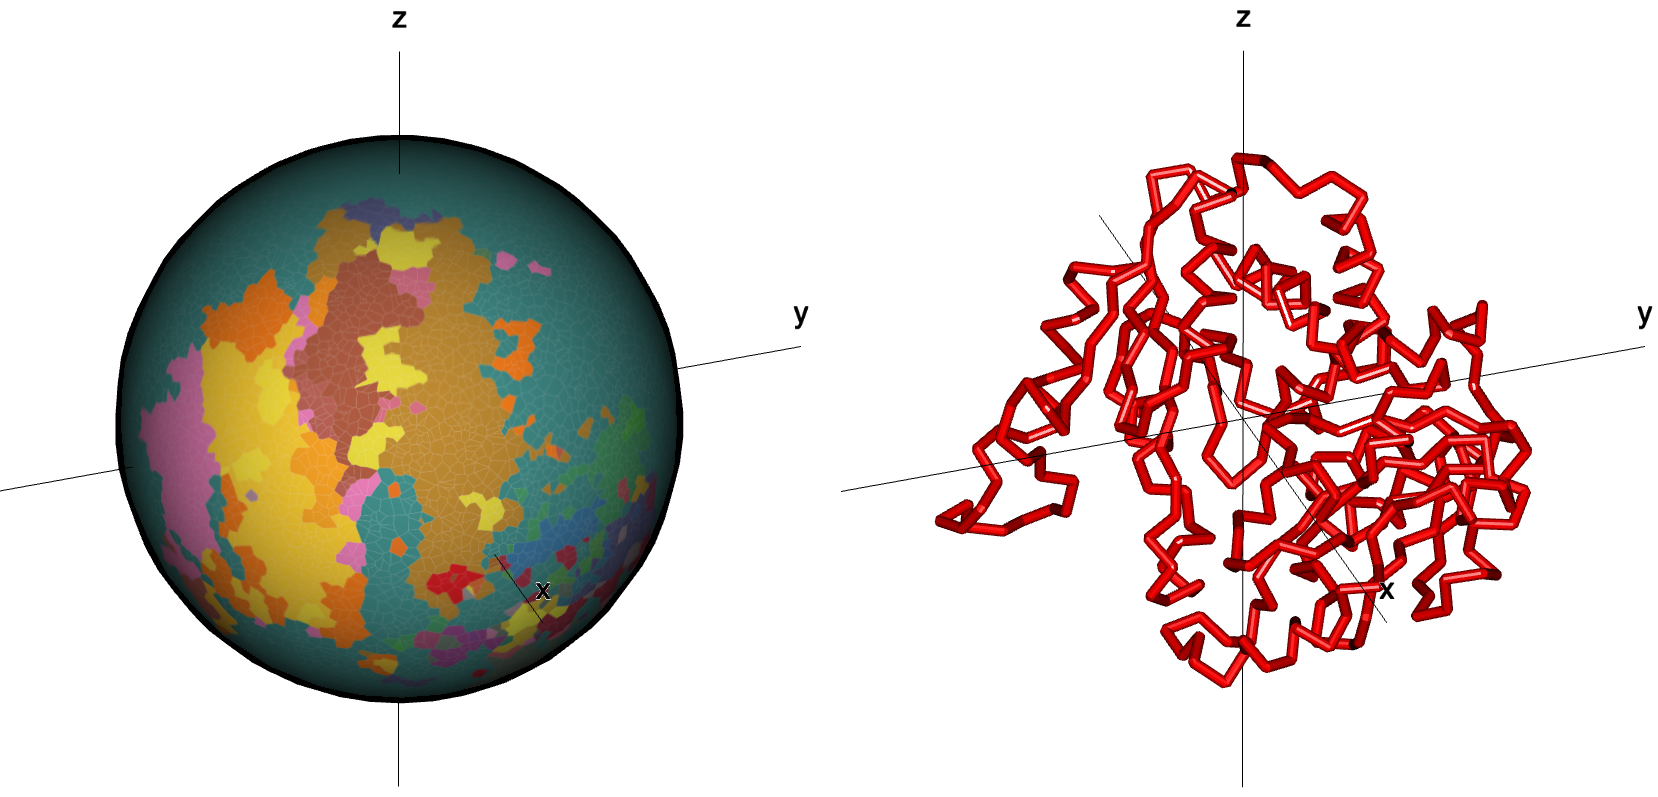
\includegraphics[width=1\textwidth]{3KZN_projection_map_3D.png}
\caption{3D projection map and backbone of the protein 3KZN, generated with the script \lstinline{plot_projection_map.R} using 10000 projections. Color corresponds to polynomial.}\label{fig:3KZN:projectionmap:3D}
\end{figure}


\subsubsection{Knots}
In order to analyze an open protein chain using knots, one works in an analogous way. Since the protein chain is an open 3D curve, we have to specify what method should be used to close the curve. At the moment the program supports two closure methods: ``direct'' and ``rays''\footnote{more details on these methods can be found in section ``\ref{sec:theory:knotoidsandcurves} \nameref{sec:theory:knotoidsandcurves}''.}. These can be specified by adding the option \lstinline{--closure-method=direct} for the former and \lstinline{--closure-method=rays} for the latter.
\begin{lstlisting}
$ bin/polynomial_invariant --closure-method=rays --names-db=internal \
  examples/3KZN_chain_A.xyz
\end{lstlisting}

The choice of projection directions can be specified with \lstinline{--nb-projections} or \lstinline{--projections-list} as discussed above. However, since the \lstinline{direct} closure (\lstinline{--closure-method=direct}) does not depend on the direction of projection, using multiple projections should only be used with \lstinline{--closure-method=rays}.

\subsubsection{Subchains, knotted cores and fingerprint matrices}
We would like now to analyze the subchains of 3KZN's backbone using the \lstinline{knotted_core} program. We start by calling
\begin{lstlisting}
$ bin/knotted_core examples/3KZN_chain_A.xyz 
\end{lstlisting}
The program will search for the knotted core, which is the shortest subchain obtained by progressively altering the length of the input curve by 1 point without changing the dominant knotoid type in the process. The dominant knotoid type of each subchain is evaluated by projecting on a sphere (using \lstinline{--nb-projections=20} by default). During the run, information on the progression will be written to standard error and after completion, the knotted core will be written to standard output
\begin{lstlisting}
#index_first  index_last  length  frequency  polynomial
168           252         85      0.5        - A^(-16) + A^(-12) + A^(-4)
170           254         85      0.45       - A^(-16) + A^(-12) + A^(-4)
\end{lstlisting}
Each line corresponds to a possible knotted core. Here, two subchains have the same the minimal length. Note that this list of possible knotted cores may change due to the random sampling of the 20 projection directions. The first knotted core is the subchain with starting index 168 (using zero-based indexing) and ending index 252 and it has a dominant polynomial invariant $-A^{-16}+A^{-12}+A^{-4}$ that appears in 50\% of the projections\footnote{see section ``\ref{sec:format:listsubchains} \nameref{sec:format:listsubchains}'' for more information on the file format.}. The second solution starts at index 170, ends at index 254 and has the same dominant polynomial invariant that appears in 45\% of the projection.

In analogy with the case explained above, we can specify the number of random projections that we want our sample to include (\lstinline{--nb-projections} or \lstinline{--projections-list}), the knot or knotoid names (\lstinline{--names-db}), the option of evaluating the diagrams on the plane (\lstinline{--planar}), the closure method (\lstinline{--closure-method}) and so on. For example, the following finds the knotted core of 3KZN using a set of predetermined projection directions and also loads the knotoid names database:
\begin{lstlisting}
$ bin/knotted_core --projections-list=examples/projections_list_100.txt \
  --names-db=internal examples/3KZN_chain_A.xyz
\end{lstlisting}
When the option \lstinline{--names-db} is used, the output has an additional column with the knot(oid) type corresponding to the dominant polynomial invariant (here 3\_1m):
\begin{lstlisting}
#index_first  index_last  length  frequency  knotoid_type  polynomial
170           252         83      0.260337   3_1m          - A^(-16) + A^(-12) + A^(-4)
\end{lstlisting}



We proceed and ask \lstinline{knotted_core} to produce all data required to generate the fingerprint matrix of 3KZN (using options \lstinline{--output-all}, \lstinline{--output-search} and \lstinline{--output}). WARNING: evaluating all subchains (option \lstinline{--output-all}) can be very slow\footnote{On a MacBook Pro from 2011 with 2.4 GHz Intel Core i5 CPU, it takes approximately 15 minutes to execute this command.}.
\begin{lstlisting}
$ bin/knotted_core --names-db=internal \
  --output-all=3KZN_all.txt --output-search=3KZN_search.txt \
  --output=3KZN_knotted_core.txt --timeout=1 examples/3KZN_chain_A.xyz
\end{lstlisting}
The option \lstinline{--timeout=1} was used to interrupt the evaluation of the polynomial after 1 second. Indeed, for a few subchains and projections, the resulting diagram has a large number of crossings and the evaluation of the polynomial invariant may be very slow. Note that if the evaluation of a polynomial invariant takes more than 1 second, the knot type and polynomial invariant are set to \lstinline{TIMEOUT}. This special value is treated as any other polynomial invariant and knot type and will appear in the output if it is the dominant knot type.

Subsequently we call the {\ttfamily R} script that creates the fingerprint matrix:
\begin{lstlisting}
$ scripts/plot_knotted_core.R --output=3KZN_fingerprint_matrix.png 3KZN_all.txt
\end{lstlisting}
To overlay the knotted core(s) (yellow circle):
\begin{lstlisting}
$ scripts/plot_knotted_core.R --output=3KZN_fingerprint_matrix.png \
  --knotted-core=3KZN_knotted_core.txt 3KZN_all.txt 
\end{lstlisting}
The resulting fingerprint matrix is shown in Figure~\ref{fig:3KZN:fingerprint}.
\begin{figure}[t]
\centering
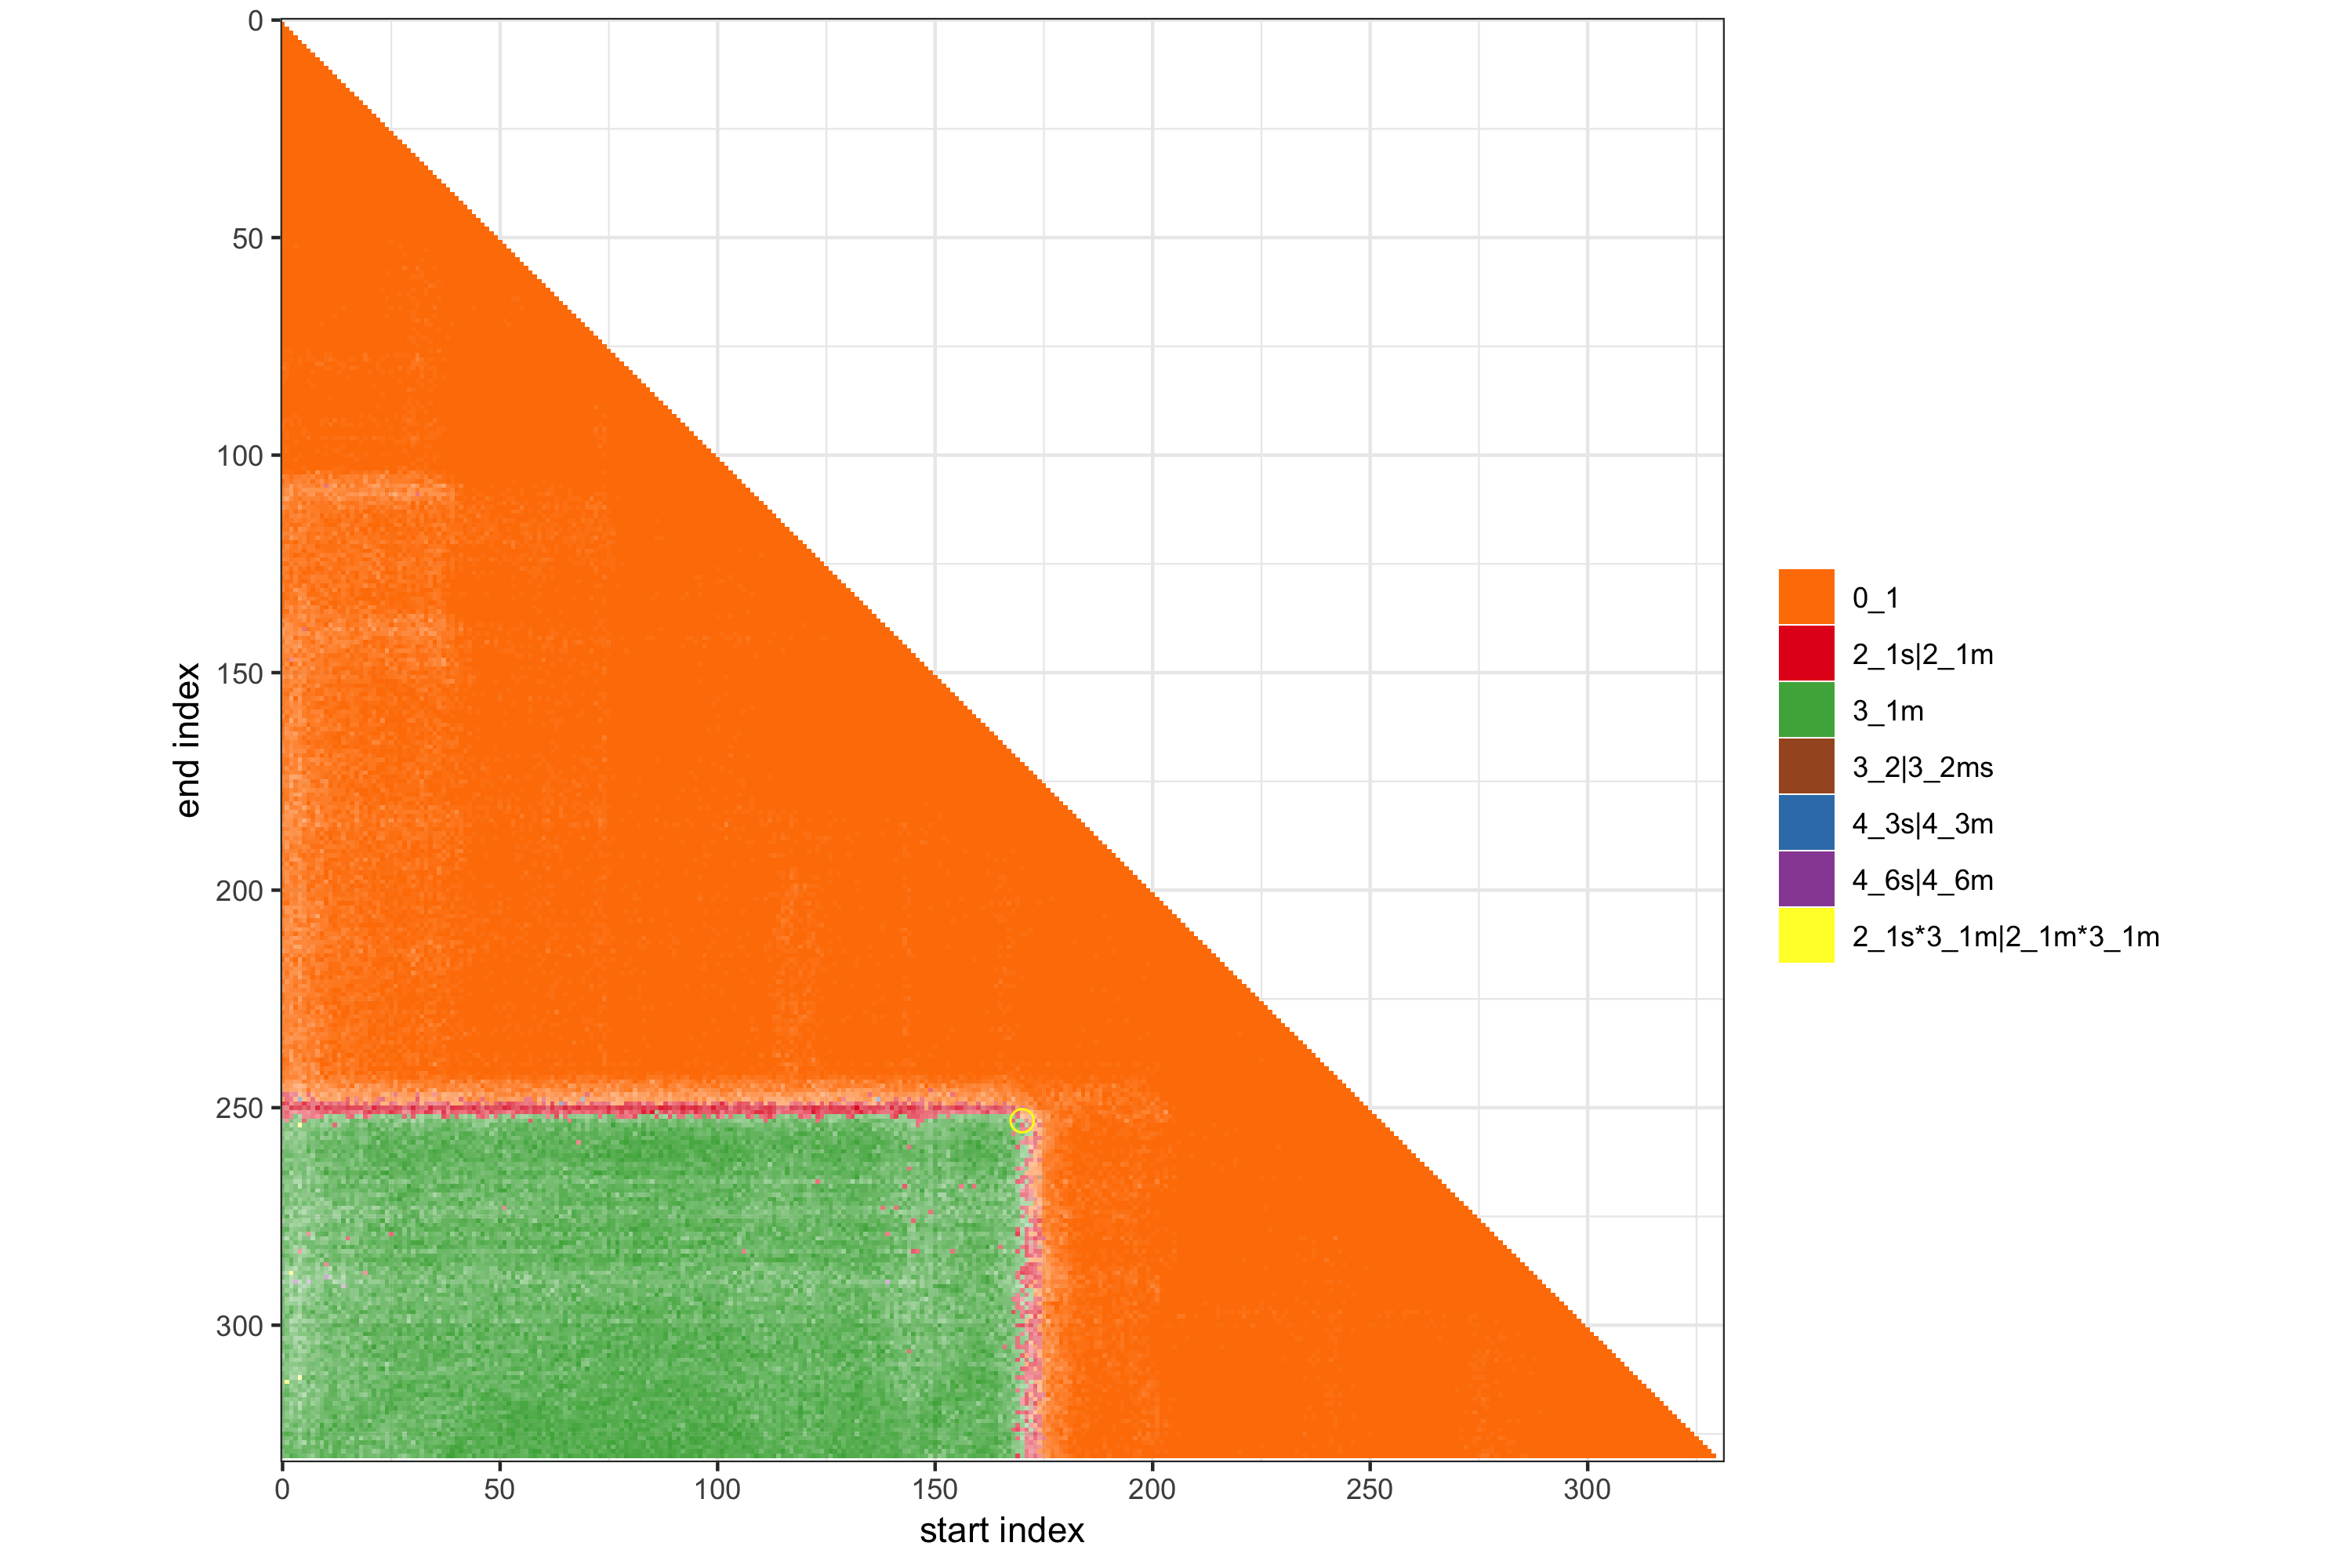
\includegraphics[width=0.9\textwidth,trim={200px 0 250px 0},clip]{3KZN_fingerprint_matrix.png}
\caption{The knotoid fingerprint matrix for the protein 3KZN. This proteins forms a deep trefoil knotoid (bottom left corner corresponds to the full chain). Color corresponds to dominant knotoid type of the subchain and transparency corresponds to its frequency. Yellow circles are centered on knotted core(s).}\label{fig:3KZN:fingerprint}
\end{figure}
The fingerprint matrix is dominated by 0\_1, 2\_1m and 3\_1m knotoids. However, because of the random sampling of a small number of projection directions used to estimate the dominant knotoid type (\lstinline{--nb-projections=20} by default), the figure has a high level of noise and several other knotoid types appear in the regions where the frequency of the dominant knotoid type is low. To decrease the level of noise, one possibility is to increase the number of projections. Figure~\ref{fig:3KZN:fingerprint1000} presents the same fingerprint matrix as in Figure~\ref{fig:3KZN:fingerprint} but obtained with \lstinline{--nb-projections=1000}. As expected, increasing the number of projections strongly decreases the level of noise, and only three dominant knotoid types remain (0\_1, 2\_1m and 3\_1m). In addition, a unique and shorter knotted core could be found (starting index 170, ending index 253, appearing in 31\% of the projections).
Obviously, increasing the number of projection not only increases the accuracy of the resulting fingerprint matrix, but it also increases the computational cost, which can quickly become prohibitively high. Therefore, it may be worth keeping the number of projection low to obtain a first approximation of the fingerprint matrix, which may be sufficient for most applications (compare Figure~\ref{fig:3KZN:fingerprint} and Figure~\ref{fig:3KZN:fingerprint1000}). 
\begin{figure}[t]
\centering
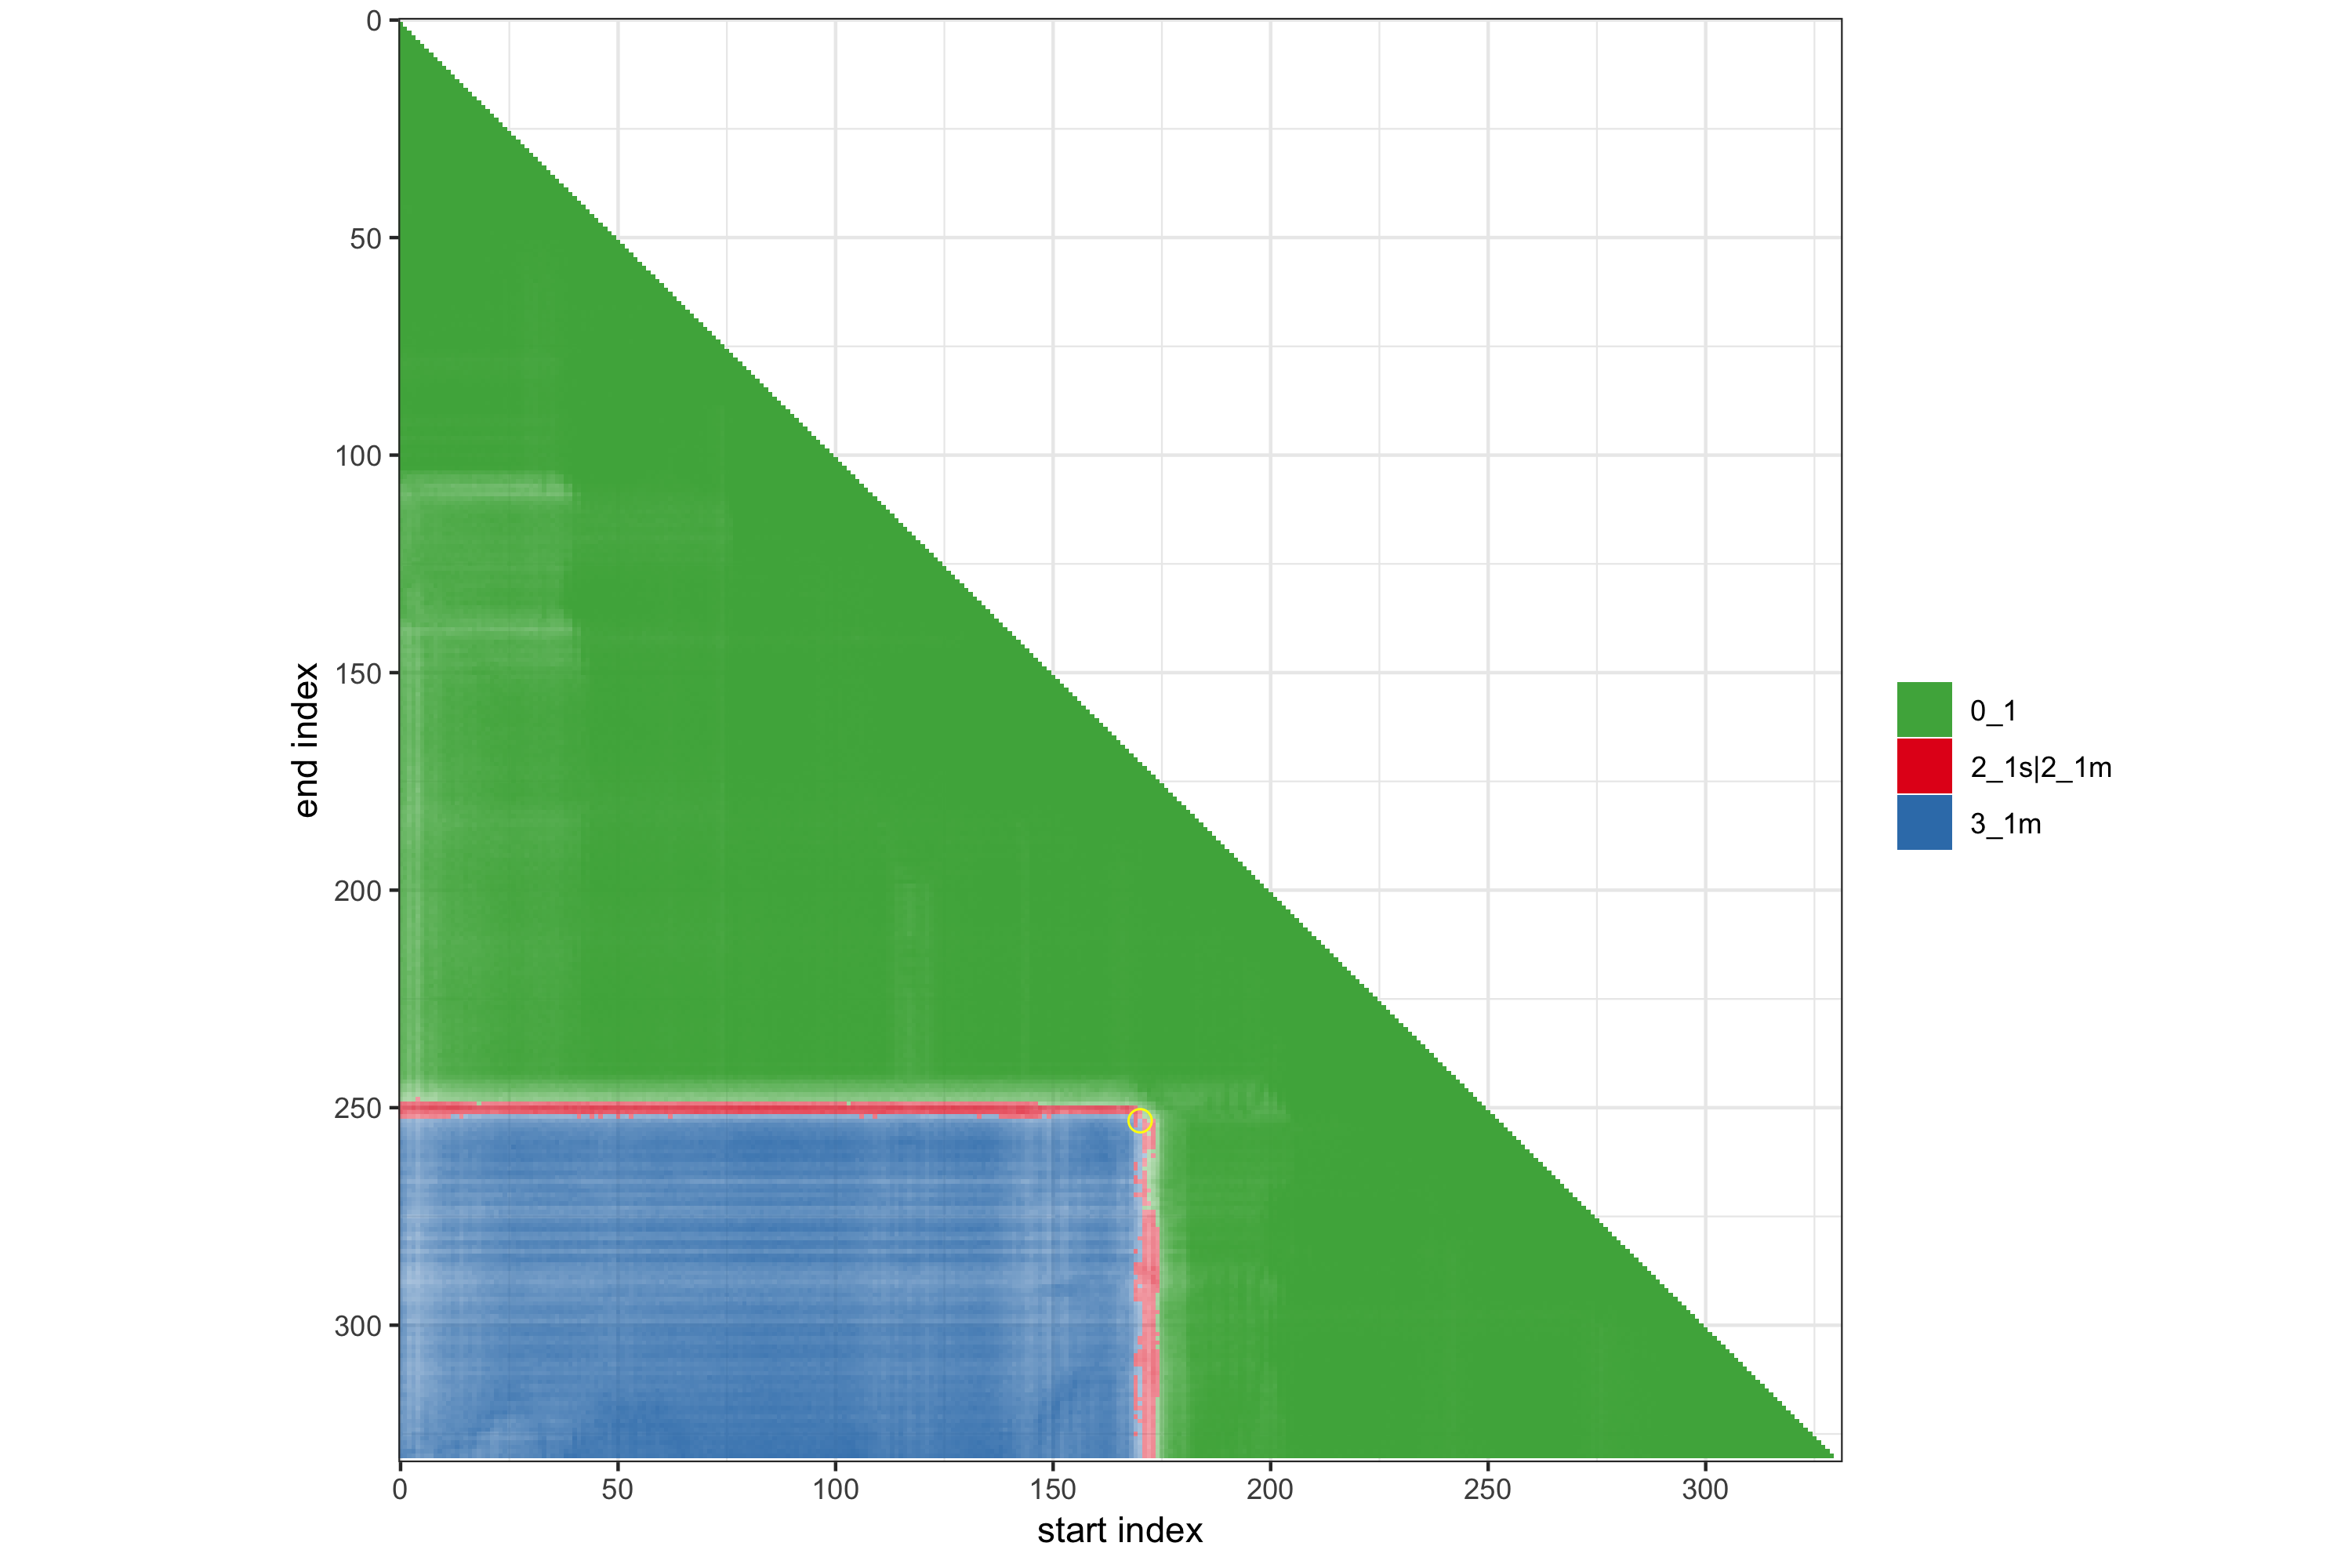
\includegraphics[width=0.9\textwidth,trim={200px 0 250px 0},clip]{3KZN_fingerprint_matrix_1000.png}
\caption{The knotoid fingerprint matrix for the protein 3KZN obtained with \lstinline{--nb-projections=1000}. A yellow circle is centered on the knotted core.}\label{fig:3KZN:fingerprint1000}
\end{figure}

Finally, we ask \lstinline{knotted_core} to produce the disk matrix of 3KZN. Since the endpoints of the chain are very close, there is no problem with connecting them with a straight line and to consider the input curve as circular (option \lstinline{--cyclic-input}). In addition, we ask \lstinline{knotted_core} to close each subchain with the \lstinline{rays} closure method\footnote{see section ``\ref{sec:theory:knotoidsandcurves} \nameref{sec:theory:knotoidsandcurves}'' for more details.}. Please note that the closure method for the input curve (option \lstinline{--cyclic-input}) and for the subchains (\lstinline{--closure-method}) can be chosen independently. WARNING: evaluating all subchains (option \lstinline{--output-all}) can be very slow\footnote{On a MacBook Pro from 2011 with 2.4 GHz Intel Core i5 CPU, it takes approximately 50 minutes to execute this command.}.
\begin{lstlisting}
$ bin/knotted_core --cyclic-input --closure-method=rays --names-db=internal \
  --output-all=3KZN_all.txt --output-search=3KZN_search.txt \
  --output=3KZN_knotted_core.txt --timeout=1 examples/3KZN_chain_A.xyz
\end{lstlisting}

A disk matrix can be produced using \lstinline{plot_knotted_core.R} with option \lstinline{--cyclic}.  WARNING: drawing heatmaps in polar coordinate using {\ttfamily R} package {\ttfamily ggplot2}\cite{wickham2009} can be very slow\footnote{On a MacBook Pro from 2011 with 2.4 GHz Intel Core i5 CPU, it takes approximately 20 minutes to execute this command.}.
\begin{lstlisting}
$ scripts/plot_knotted_core.R --cyclic --output=3KZN_circular_matrix.png \
  --knotted-core=3KZN_knotted_core.txt 3KZN_all.txt
\end{lstlisting}
The resulting disk matrix is shown in Figure~\ref{fig:3KZN:disk}
\begin{figure}[t]
\centering
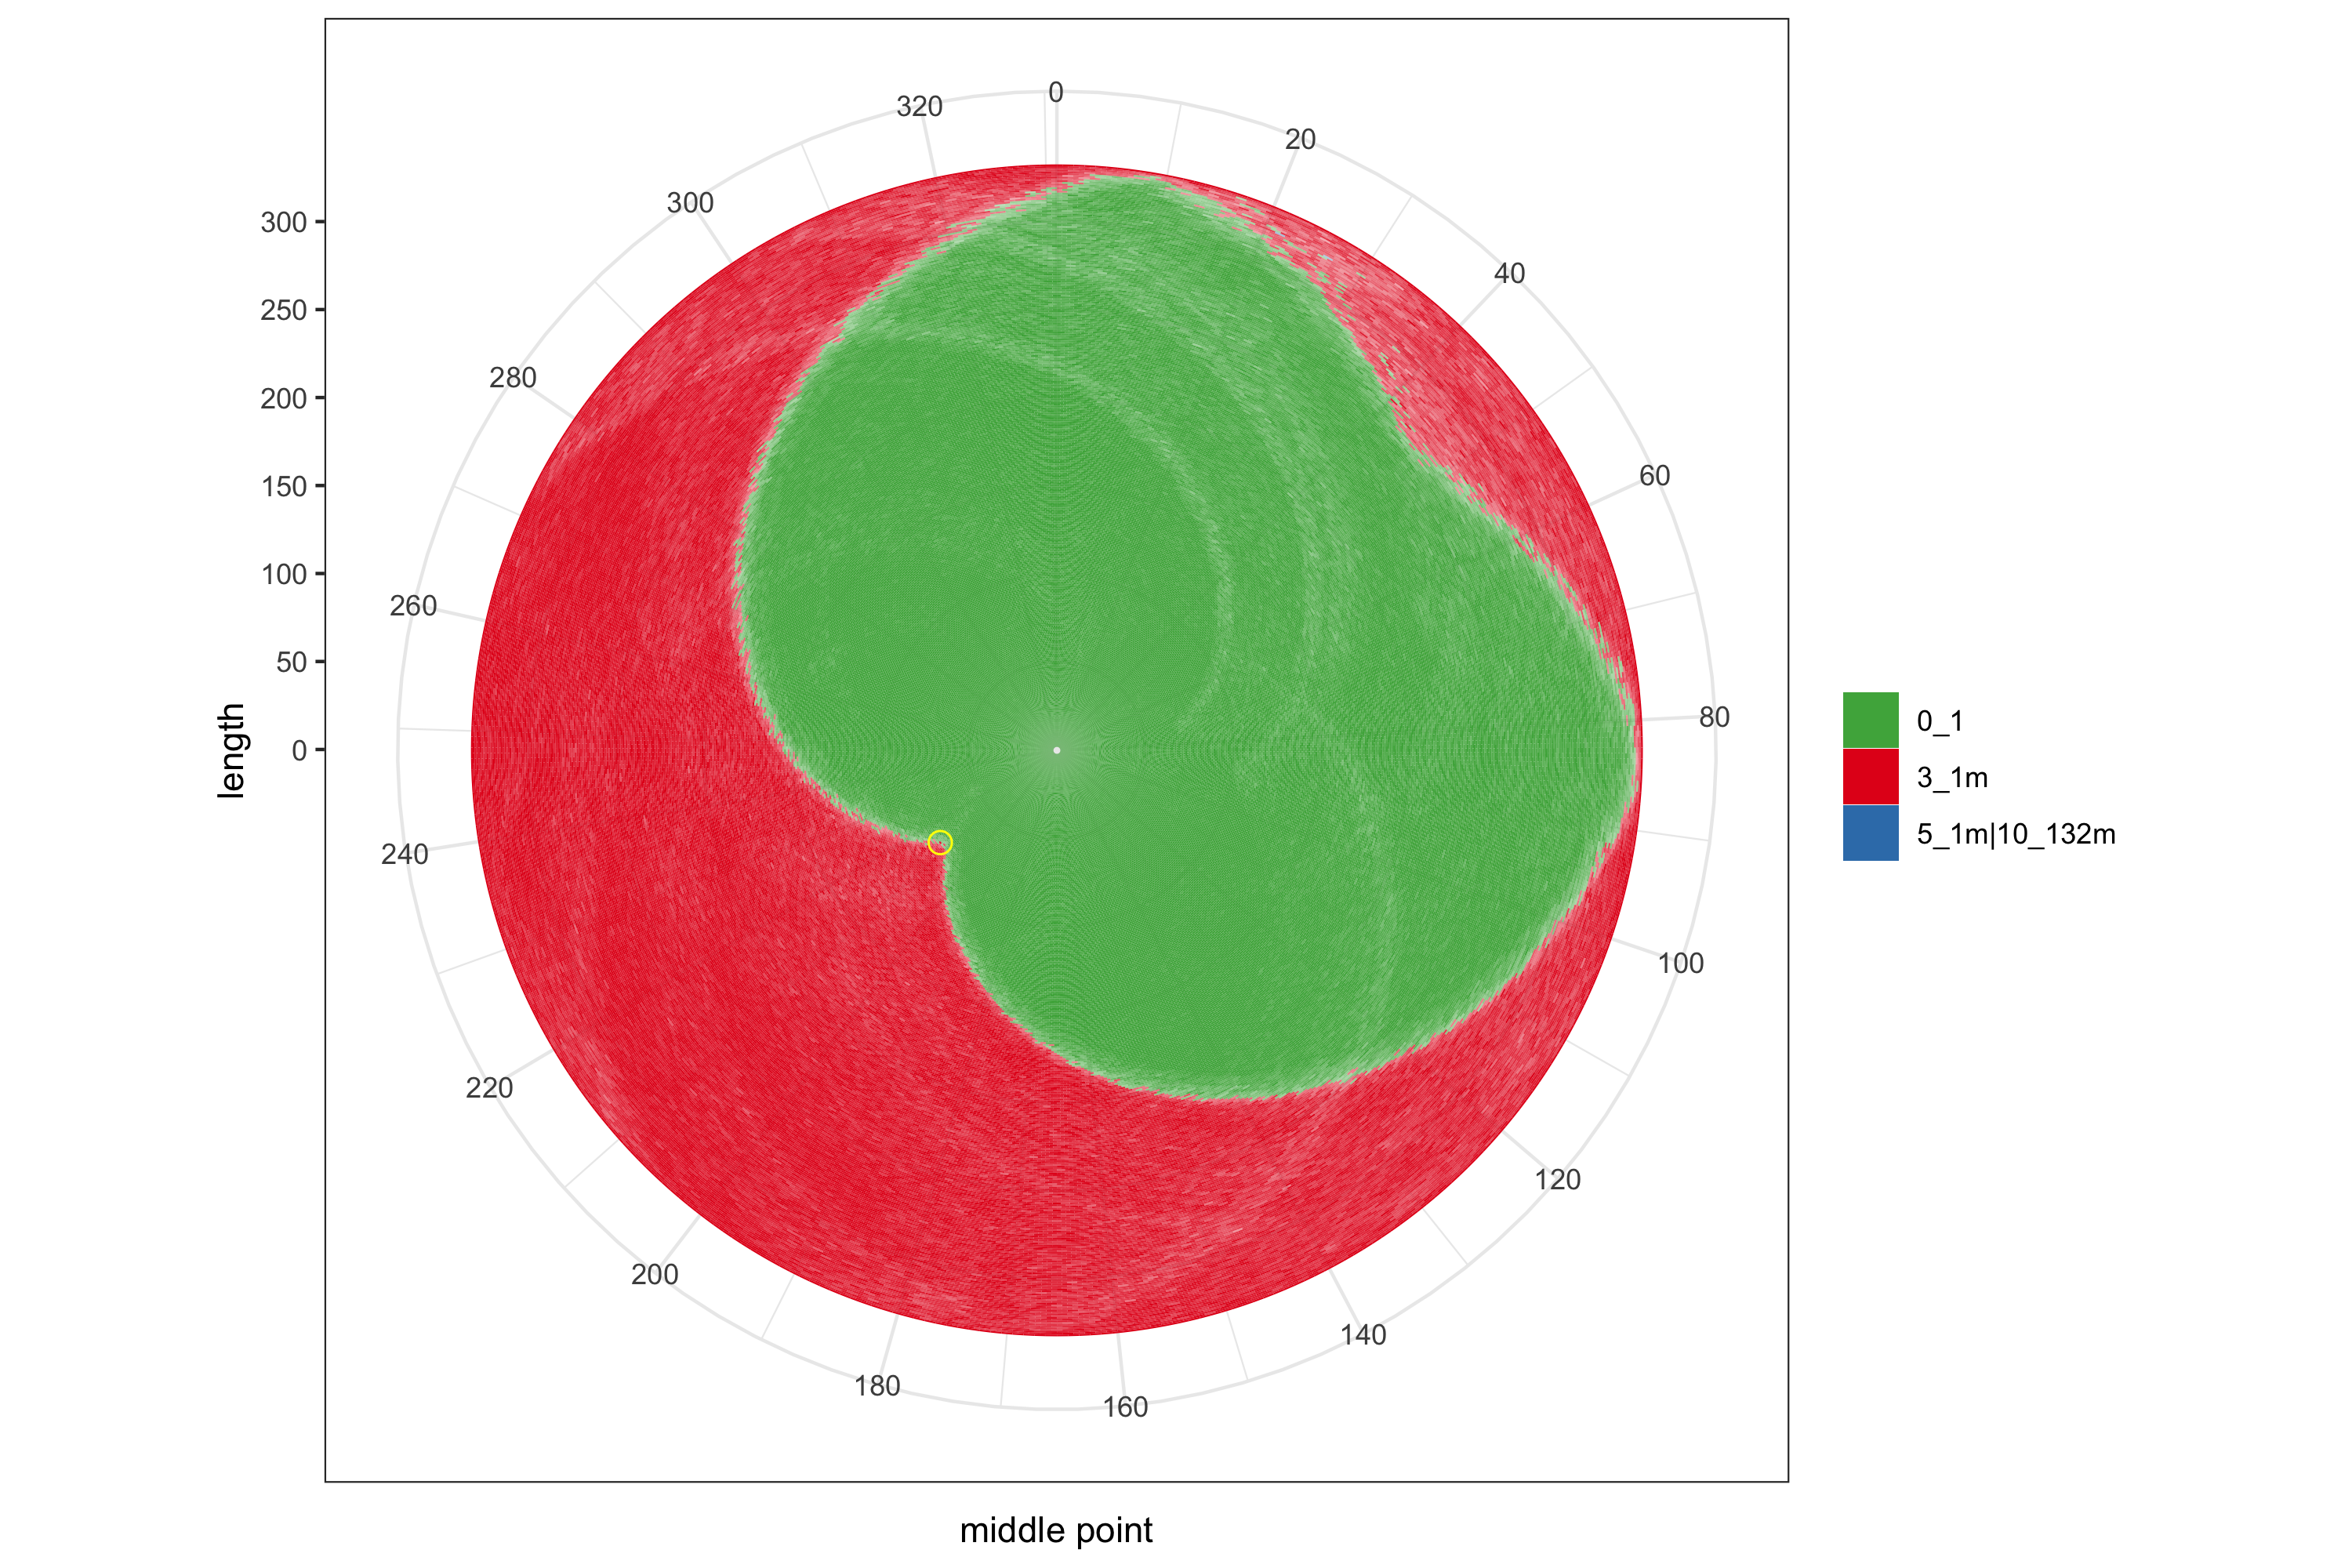
\includegraphics[width=0.9\textwidth,trim={280px 0 300px 0},clip]{3KZN_circular_matrix.png}
\caption{The disk matrix for the protein 3KZN with uniform closure (i.e. \lstinline{--closure-method=rays} in multiple directions). This proteins forms a right handed trefoil knot (all points on the enclosing circle corresponds to the full chain). Color corresponds to dominant knot type of the subchain and transparency corresponds to its frequency. Yellow circles are centered around knotted core(s).}\label{fig:3KZN:disk}
\end{figure}



\clearpage
